%!TEX TS-program = xelatex
%!TEX encoding = UTF-8 Unicode
%!BIB TS-program = biber
%!BIB program = biber

\documentclass[a4paper,11pt,twoside,headsepline]{scrbook}

\usepackage[spanish,es-tabla,es-noshorthands,es-ucroman]{babel}
\usepackage{xltxtra}
\usepackage{fontspec}
\usepackage{xunicode}
\usepackage{amsmath}
\usepackage{amsthm}
\usepackage[top=3cm,bottom=3cm,outer=3cm,inner=2cm]{geometry}
\usepackage[Bjornstrup]{fncychap}
\usepackage{graphicx}
\usepackage{amssymb}
\usepackage[breaklinks=true]{hyperref}
\def\UrlBreaks{\do\/\do-\do.}
\usepackage{hyperxmp}
\usepackage{enumerate}
\usepackage{siunitx}
\usepackage{float}
\usepackage{mdwlist}
\usepackage[table,usenames,dvipsnames]{xcolor}
\usepackage{titlesec}
%\usepackage{subfigure}
\usepackage[autostyle]{csquotes}
\usepackage[style=authoryear,natbib=true,%
maxbibnames=99,maxcitenames=2,%
citestyle=authoryear-comp,doi=true,url=true,backend=biber,dashed=no]{biblatex}
\bibliography{\jobname}
\usepackage[hypcap]{caption}
\usepackage{epigraph}
\usepackage{framed}
\usepackage{dcolumn}
\usepackage{pdflscape}
\usepackage{booktabs}
\usepackage{subcaption}
\usepackage{hhline}
\usepackage{multirow}
\usepackage{afterpage}
\usepackage[multiple]{footmisc}
\usepackage{pdfpages}

\usepackage[section]{placeins}

\usepackage[colorinlistoftodos, shadow]{todonotes}
  \presetkeys{todonotes}{inline}{}
\usepackage{morewrites} % problem with todolist 

\usepackage{makeidx}\makeindex
\usepackage{pifont}% http://tex.stackexchange.com/questions/42619/x-mark-to-match-checkmark
\newcommand{\cmark}{{\color{OliveGreen}\ding{51}}}
\newcommand{\xmark}{{\color{red}\ding{55}}}

\theoremstyle{definition}
\newtheorem{definition}{Definición}[chapter]

\theoremstyle{definition}
\newtheorem{example}{Ejemplo}[chapter]

\usepackage{menukeys}
\usepackage{csvsimple}

%% plantuml %%
\usepackage{filecontents}
\usepackage{tikz}
\usetikzlibrary{calc}

\sisetup{output-decimal-marker={.},
	group-digits=true,
	group-minimum-digits={3},
	group-separator = \text{\,},
	product-units=single,
	detect-all, detect-inline-family=text, detect-inline-weight=text,
  detect-display-math=true}

\hyphenation{%
WordNet
frame-work
}

%% minted %%
\makeatletter
\renewcommand\fs@ruled{\def\@fs@cfont{\bfseries}\let\@fs@capt\floatc@ruled
  \def\@fs@pre{\hrule height.8pt depth0pt \kern2pt}%
  \def\@fs@post{\vskip-0.7\baselineskip\kern2pt\hrule\relax}%
  \def\@fs@mid{\kern2pt\hrule\kern2pt}%
  \let\@fs@iftopcapt\iftrue}
\makeatother
\floatstyle{ruled}
\usepackage[chapter]{minted}
\newcommand{\codep}[2][python]{%
	\mintinline{#1}{#2}%
}
\newcommand{\codet}[2][text]{%
	\mintinline[escapeinside=@@]{#1}{#2}%
}
\renewcommand{\listingscaption}{Código}
\providecommand*{\listingautorefname}{\listingscaption}
\renewcommand{\listoflistingscaption}{Índice de códigos}
\setminted{breaklines=true,linenos=true}

\newcommand*{\fullref}[1]{\hyperref[{#1}]{\autoref*{#1}: ``\nameref*{#1}''}}

%% estilo %%

\defaultfontfeatures{%Mapping=tex-text,
  Numbers={Lining}}
\setmonofont[Scale=0.8]{Menlo}
\newfontfamily\portadafont{Arial Bold}
%\DefineBibliographyStrings{spanish}{andothers={et~al\adddot}}
\newfontfamily\nombrefont{Futura}[Scale=0.94]
\newcommand{\nombrebf}[1]{\textbf{\sffamily #1}}
\newcommand{\nombre}[1]{\begingroup\nombrefont #1\endgroup}
\setromanfont[Mapping=tex-text]{Hoefler Text}
%\setsansfont[Scale=MatchLowercase,Mapping=tex-text]{Gill Sans}
%\setmonofont[Scale=0.9]{Courier New}


\DeclareMathOperator*{\argmin}{arg\,min}
\DeclareMathOperator*{\argmax}{arg\,max}

%\setlength{\parindent}{2em}
\setlength{\parskip}{1em plus4mm minus3mm}
\linespread{1.1}

%% reduce widows
\makeatletter
\@beginparpenalty=10000
\makeatother
\clubpenalty=8000
\widowpenalty=6000
%\usepackage{parskip}

%% doc info %%
\newcommand{\pfctitle}{Procesamiento del Lenguaje Natural aplicado al Análisis del Sentimiento de opiniones}
\newcommand{\pfcauthor}{Guillermo Gutiérrez-Herrera}
\newcommand{\pfcdate}{septiembre de 2015}

\title{\pfctitle}
\author{\pfcauthor}
\date{\pfcdate}

\hypersetup{
  pdftitle=\pfctitle,
  pdfauthor=\pfcauthor,
  pdfkeywords={Natural Language Processing, Machine Learning, Sentiment Analysis},
  pdfcontactemail={guiguther@alum.us.es},
  pdflang={es},
}

\usepackage{txstd830}

\begin{document}

\frontmatter

\pagenumbering{gobble}
\clearpage
%!TEX root = pfc-memoria.tex
%!TEX encoding = UTF-8 Unicode

\thispagestyle{empty}

\begingroup

\begin{center}

\includegraphics[width=4cm]{logo_us}\\[1.3cm]

\Large

\portadafont

ESCUELA TÉCNICA SUPERIOR DE INGENIERÍA INFORMÁTICA\\[0.8cm]

INGENIERO EN INFORMÁTICA (Plan 97)\\[2.8cm]

\MakeUppercase{\pfctitle}\\[2.7cm]

\large

Realizado por\\[0.1cm]

\MakeUppercase{\pfcauthor}\\[0.8cm]

Dirigido por\\[0.1cm]

JOSÉ ANTONIO TROYANO\\[0.8cm]

Departamento\\[0.1cm]

LENGUAJES Y SISTEMAS INFORMÁTICOS\\[3.6cm]


\end{center}

\begin{flushright}
\portadafont
Sevilla, \pfcdate
\end{flushright}

\endgroup


\cleardoublepage
\pagenumbering{roman}
%!TEX root = pfc-memoria.tex
%!TEX encoding = UTF-8 Unicode

\thispagestyle{plain}
\section*{Agradecimientos}

Este trabajo no hubiera sido posible sin la inestimable ayuda de mi tutor, José Antonio Troyano, que me ha guiado tanto en la concepción del proyecto como en la consecución de los objetivos, y a quien le agradezco su enorme paciencia y confianza.

Agradezco en general a todos los profesores de la titulación, especialmente del departamento de Lenguajes y Sistemas Informáticos, hacer las clases amenas y las asignaturas interesantes y accesibles.

A mis compañeros de trabajos en grupo de las distintas asignaturas, que hemos sabido trabajar bien para conseguir buenas notas: Carlos Herce (\href{https://twitter.com/charlosherce}{@CharlosHerce}) y Jesús Corral Pérez.

Así también agradezco el apoyo y compresión de mi familia, que han tenido que sufrir dos PFC, el anterior de la Ingeniería Técnica y éste de la Ingeniería Superior. En especial a mi abuelo Juan Antonio Herrera por transmitirme sus conocimientos sobre el trabajo del ingeniero, y sobre la vida.

A Carmen Dorantes,\footnote{\url{https://palabrasdemandragora.wordpress.com/}} la persona que significó mucho en mi vida, también le dedico este trabajo; por enseñarme a ser feliz.


\cleardoublepage
\tableofcontents

\mainmatter

%% %% %% %% %% %% %%

%!TEX root = pfc-memoria.tex
%!TEX encoding = UTF-8 Unicode

\cleardoubleevenemptypage
\part{Introducción y objetivos}
\label{part:introduccion-objetivos}

%!TEX root = pfc-memoria.tex
%!TEX encoding = UTF-8 Unicode

\chapter{Introducción}

Durante la carrera tenemos asignaturas que tratan sobre procesamiento de lenguajes, pero siempre lenguajes formales. El lenguaje natural es mucho más complejo y ambiguo, y difícil de procesar.


\begin{definition}[NLP]\index{NLP}\index{procesamiento del lenguaje natural}\index{natural language processing@\emph{natural language processing}}
El procesamiento de lenguaje natural (PLN, o NLP del inglés \emph{Natural Language Processing}) es el campo de ciencias de la computación, inteligencia artificial y lingüística que estudia las interacciones entre las computadoras y el lenguaje humano \citep[Procesamiento de lenguajes naturales]{wikipedia-es}.
\end{definition}

Para conseguir procesar el lenguaje natural de forma eficiente se debe proveer a las computadoras de herramientas para comprender el conocimiento humano expresado en lenguaje natural (voz o texto, principalmente), y saber representarlo.

En regla general, el lenguaje natural es abierto a interpretaciones, de manera que los resultados de estas técnicas no pueden ser 100\% exactos siempre, y aceptaremos resultados parciales y aproximaciones.

Con la aparición de la denominada \nombrebf{Web 2.0}, las páginas dinámicas, y los gestores de contenido web, los consumidores de información (usuarios o visitantes de páginas web) son también productores de la información. Estos usuarios producen en su mayoría contenido de tipo texto, obviamente en lenguaje entendible por otros humanos, con poca capacidad para el \emph{software} de realizar cualquier cálculo, extracción, comprensión, o modificación al mismo en documentos sin una estructura formalizada previa ni preparados para ser consumido por la máquinas. En el estudio de \citet{Hilbert2011}, se estima cuál es la capacidad global de información generada, en su tramo analógico y digital a lo largo del tiempo, observando una explosión digital a partir del año 2002 (\autoref{fig:InfoGrowth}).

De esta manera, ha suscitado un mayor interés por la comunidad científica en aprovechar esa vasta cantidad de información disponible para comprender los datos y extraer información útil resumida de ellos y con alguna aplicabilidad, en las llamadas tareas de \nombrebf{minería de datos} (en inglés: \emph{data mining}).\index{minería!de datos}\index{data mining}

En el caso del análisis de textos: \nombrebf{minería de textos}.\index{minería!de textos}\index{text mining}

\begin{landscape}
\begin{figure}[htbp]
\centering
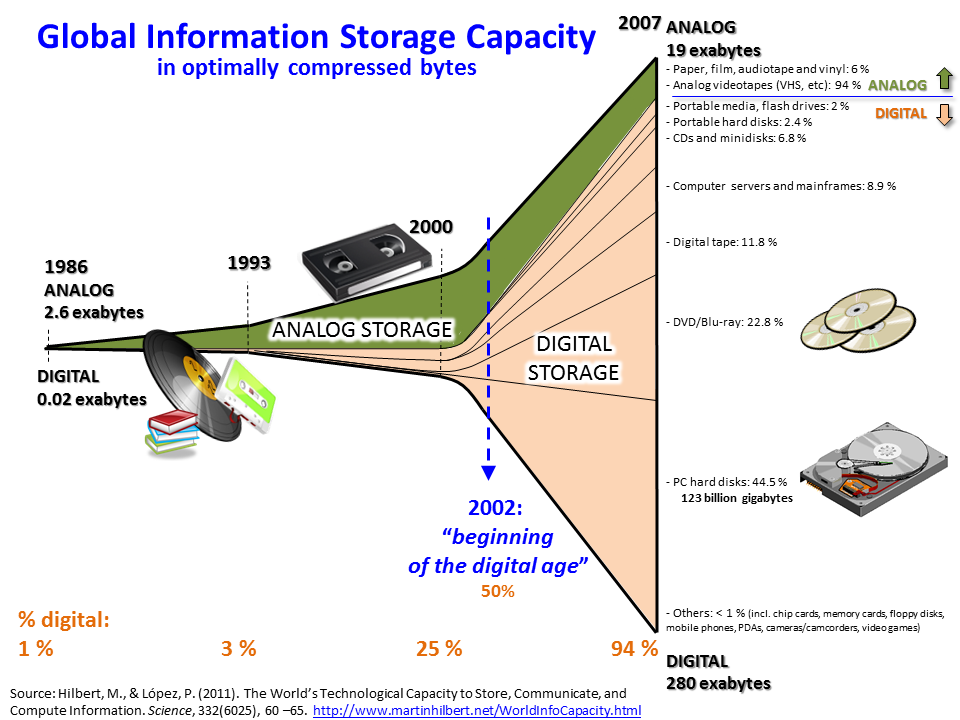
\includegraphics[height=0.85\textwidth]{Hilbert-InfoGrowth}
\caption[Explosión de información digital]{Gracias a la \nombrebf{explosión de información digital}, existe actualmente gran cantidad de información disponible para extraer el conocimiento humano, inclusive el lenguaje natural, de manera automática, por las máquinas \citep{Hilbert2011}. \\
{\footnotesize ``Hilbert InfoGrowth'' by Myworkforwiki - Own work. Licensed under CC BY-SA 3.0 via Wikimedia Commons - \url{https://commons.wikimedia.org/wiki/File:Hilbert_InfoGrowth.png\#/media/File:Hilbert_InfoGrowth.png}}}
\label{fig:InfoGrowth}
\end{figure}
\end{landscape}

\section{Sentimiento o polaridad de las opiniones}

En los documentos de tipo crítico, o comentarios de opinión acerca de una película, un artículo o un servicio, la información que se extrae de su lectura es si la película, el artículo o el servicio le ha parecido bueno o malo. A esto se le llama la \nombrebf{polaridad del sentimiento}\index{polaridad!sentimiento}\index{sentimiento}\index{polaridad} (o simplemente sentimiento) de la crítica. Se puede ver un ejemplo de escala de valoración de esta polaridad (con varias graduaciones entre positivo y negativo) en la \autoref{fig:tramos-polaridad}.

\begin{figure}[htbp]
\centering
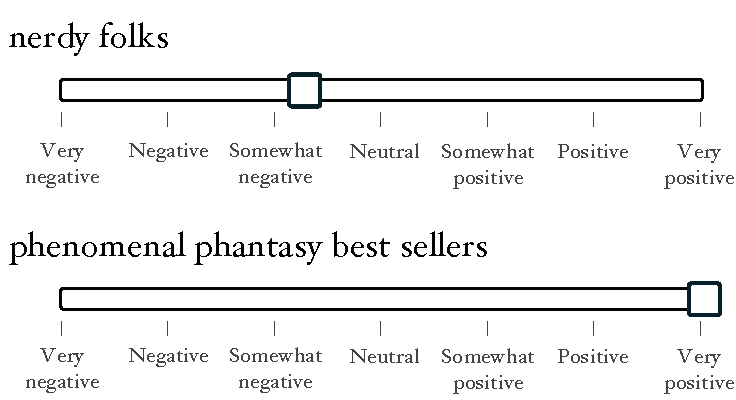
\includegraphics[height=5.5cm]{tramos-polaridad}
\caption[Escala de valoración del sentimiento en Penn Sentiment Treebank]{Escala de valoración del sentimiento empleada en el proyecto Penn Sentiment Treebank de la Universidad de Pennsylvania \citep{Socher2014}}
\label{fig:tramos-polaridad}
\end{figure}


En las páginas dedicadas a opiniones de productos en general como \nombre{Ciao!}\footnote{\url{http://www.ciao.es/}}, o más específicamente para críticas de cine como \nombre{FilmAffinity}\footnote{\url{http://www.filmaffinity.com/}}, se suele proporcionar al usuario un formulario para introducir un texto con su crítica, y además un elemento para que etiquete su valoración, bien en una escala de puntuación o bien mediante estrellitas.

\begin{figure}[htbp]
\centering
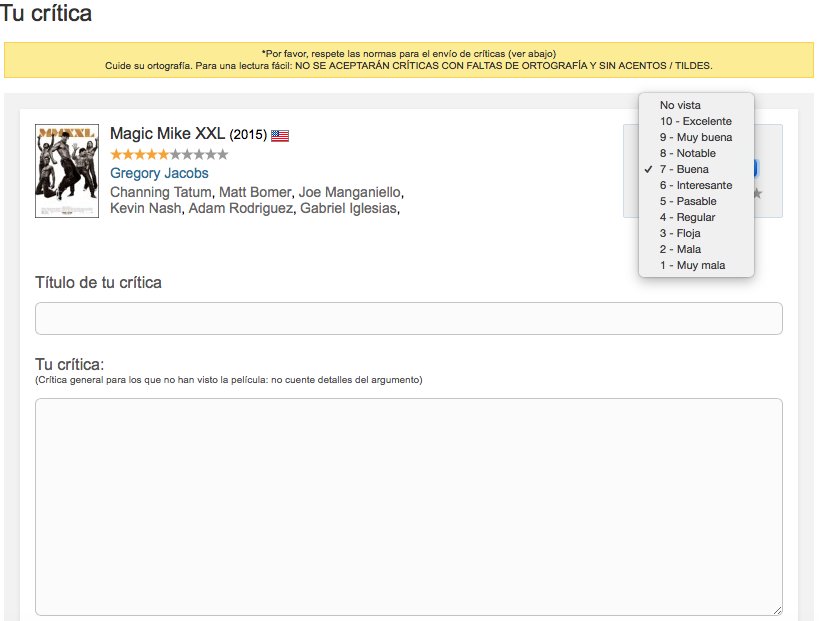
\includegraphics[width=0.95\textwidth]{filmaffinity}
\caption[Introducción de la valoración en FilmAffinity]{En FilmAffinity han optado por el desplegable de 1 a 10 puntos etiquetados para introducir la valoración.}
\label{fig:filmaffinity}
\end{figure}

\begin{figure}[htbp]
\centering
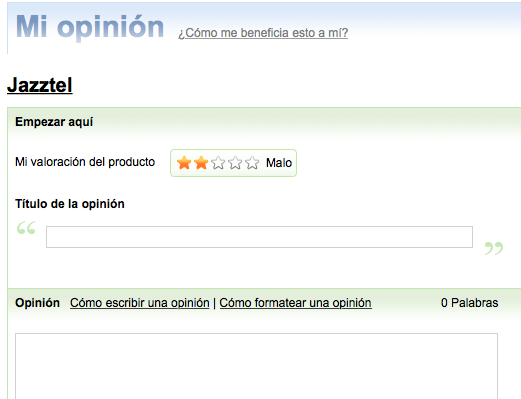
\includegraphics[width=0.7\textwidth]{ciao}
\caption[Introducción de la valoración en ciao.es]{Introducción de la valoración en ciao.es, con estrellitas.}
\label{fig:ciao}
\end{figure}

En este tipo de documentos es fácil determinar cuál es la polaridad del texto de la crítica, pues tenemos disponible además un campo de tipo numérico o enumerado (numérico en el sentido de ser inmediatamente procesable por la máquina, sin mayor tratamiento que quizás un cambio de escala o conversión de tipo entero a coma flotante) con la valoración, y podemos asociar valoraciones altas con polaridad buena o muy buena, y las valoraciones bajas con polaridad mala o muy mala. Las valoraciones medias se asociarían a comentarios cuya polaridad del sentimiento será neutra.

\section{Motivación}

Con el amplio uso de las plataformas de twitter y Facebook, los consumidores de productos y servicios pueden criticar abiertamente mediante un comentario a las marcas de las empresas cuyos productos han gustado o no. En la vida virtual, al igual en la vida real, las personas comentamos con nuestros amigos, y recomendamos o no recomendamos estos productos, contribuyendo con nuestras experiencias a mejorar o empeorar la \nombrebf{reputación de las marcas.}\index{reputación!de marca}

Twitter se ha consolidado de esta manera como una forma digital de boca-a-boca \citep{Jansen2009}, pero con mayores posibilidades de alcanzar un gran impacto (o \nombrebf{viralidad}\index{viralidad}) al distribuirse mediante la red global de Internet, y llegar a gran cantidad de público. Es más, por nuestra naturaleza, tendemos a reproducir la mala publicidad de un compañía con mayor asiduidad que la buena publicidad, por eso las empresas deben estar presentes en las redes sociales y monitorear su \nombrebf{reputación online}\index{reputación!online} \citep{Leiva2012}.



%!TEX root = pfc-memoria.tex
%!TEX encoding = UTF-8 Unicode

\chapter{Objetivos}

Los objetivos del proyecto son

\begin{itemize}
\item Estudiar las características del lenguaje natural que lo hacen diferente del lenguaje formal.
\item Estudiar algunas estrategias, métodos, procedimientos o algoritmos para analizar y extraer información de textos en lenguaje natural.
\item Estudiar algoritmos de aprendizaje automático aplicado a tareas de NLP.
\item Desarrollar una biblioteca unificada de NLP y aprendizaje automático para el análisis del sentimiento o polaridad de opiniones.
\item Desarrollar un asistente con una Interfaz Gráfica de Usuario (IGU, \emph{GUI}) para usar en el aula.
\end{itemize}


\cleardoubleevenemptypage
\part{Investigación y estudio}
\label{part:investigacion-estudio}

%!TEX root = pfc-memoria.tex
%!TEX encoding = UTF-8 Unicode

\chapter{Procesamiento del lenguaje natural}

\section{Lenguaje natural vs lenguajes formales}

\section{Preprocesamiento}

\subsection{\emph{``Tokenización''}}

La \emph{tokenización}\index{tokenización}\index{tokenization@\emph{tokenization}} en NLP es normalmente el proceso de separar la cadena de entrada, frases en lenguaje natural, en las distintas palabras que componen la frase. Puede ser simplemente un separador que trocee la frase cada vez que se encuentre un espacio.
\begin{listing}[H]
\begin{minted}{python}
>>> 'of escapades demonstrating the adage that what is good for the goose'.split()
['of', 'escapades', 'demonstrating', 'the', 'adage', 'that', 'what', 'is', 'good', 'for', 'the', 'goose']
>>> 
\end{minted}
\caption{Tokenización sencilla mediante la separación de espacios.}
\label{lst:tokenizacion-sencilla}
\end{listing}

La tokenización en su sentido más amplio y general es el procedimiento del análisis léxico para reconocer lexemas del flujo de entrada con la que se obtiene un flujo de salida compuesto por tokens \citep[§2.2]{Jimenez2004}.

\begin{definition}[Token] \index{token}
Denominamos \emph{token} al conjunto de cadenas de caracteres con significado mínimo.
\end{definition}

\begin{definition}[Patrón] \index{patrón}
El \emph{patrón} es una regla que describe el conjunto de caracteres que cuadran un token.
\end{definition}

El concepto de ``cuadrar'' se denomina en inglés como match\index{match@\emph{match}}, y también se puede traducir como concordancia o correspondencia.

\begin{definition}[Lexema] \index{lexema}
Un \emph{lexema} es una secuencia concreta de caracteres que se corresponde con el patrón de un token determinado.
\end{definition}

\begin{example} \index{token} \index{patrón} \index{lexema}
Pongamos algunos ejemplos de tokens, patrones y lexemas, de un lenguaje formal típico de programación:
\nopagebreak
\begin{center}
\begin{tabular}{|l|l|l|}
\hline
\textbf{token} & \textbf{lexemas de ejemplo} & \textbf{descripción informal del patrón} \\ \hhline{===}
\codep{CONST} & \codep{const} & const \\ \hline
\codep{IF} & \codep{if} & if \\ \hline
\codep{OPREL} & \codep{<}, \codep{<=}, \codep{=}, \codep{>}, \codep{>=} & <~ ó <= ó = ó >~ ó >= \\ \hline
\codep{ID} & \codep{pi}, \codep{contador}, \codep{D2} & letra seguida de letras y dígitos \\ \hline
\codep{CTENUM} & \codep{3.1416}, \codep{0}, \codep{6.1E23} & cualquier constante numérica \\ \hline
\codep{LITERAL} & \codep{"core dumped"} & cualesquiera letras entre \codep{"} y \codep{"} excepto \codep{"} \\ \hline
\end{tabular}
\end{center}
\end{example}

En lenguaje natural, la unidad mínima de información textual será la palabra. De manera que token y lexema coinciden siempre, y no tiene sentido definir un patrón para cada token de las palabras de un diccionario de la lengua, ya que el patrón es la propia secuencia de letras de la palabra.

Existen distintos niveles de tokenización de documentos \citep[ch.~1]{Perkins2010}:
\nopagebreak
\begin{itemize}
\item Tokenizar textos en frases.
\item Tokenizar frases en palabras.
\end{itemize}

Simplemente para la primera tarea ya nos encontramos con dificultades, pues las frases no sólo terminan en punto. Pueden terminar en punto (\codep{.}), signo de exclamación (\codep[text]{!}), signo de interrogación (\codep[text]{?}), en algunos casos dos puntos (\codep{:}). Y en otros idiomas, como el español, también hay que tener en cuenta que en la separación entre frases puede haber signos de apertura de interrogación o exclamación, etc. Y también hay que tener en cuenta los puntos que separar unidades de millar en una cifra, o los puntos suspensivos, los puntos usados en acrónimos y abreviaturas, \ldots

En cuanto a la separación de palabras, también pueden surgir problemas, dependiendo del idioma. En el siguiente ejemplo (\autoref{lst:wordtokenizers}) podemos ver distintas formas de separar palabras de una frase en inglés que usa contracciones.\footnote{También se puede encontrar un demostrador interactivo de la tokenización en la siguiente dirección:\\
\url{http://text-processing.com/demo/tokenize/}}

\begin{listing}[H]
\begin{minted}{python}
>>> from nltk.tokenize import TreebankWordTokenizer, WordPunctTokenizer, WhitespaceTokenizer
>>> TreebankWordTokenizer().tokenize("Can't is a contraction.")
['Ca', "n't", 'is', 'a', 'contraction', '.']
>>> WordPunctTokenizer().tokenize("Can't is a contraction.")
['Can', "'", 't', 'is', 'a', 'contraction', '.']
>>> WhitespaceTokenizer().tokenize("Can't is a contraction.")
["Can't", 'is', 'a', 'contraction.']
>>> 
\end{minted}
\caption{Diferentes estrategias de separación de palabras}
\label{lst:wordtokenizers}
\end{listing}

Una mejor aproximación al problema es reemplazar --previamente a la tokenización--, las palabras contraídas con sus palabras equivalentes sin contracción.\footnote{Puede obtenerse un catálogo bastante extenso de contracciones en inglés --en uso y arcaicas--, en la dirección: \url{http://www.enchantedlearning.com/grammar/contractions/list.shtml}}
Para ello es necesario construirse una tabla que establezca el mapping \citep{Perkins2014}.

Como ejemplo de un conjunto de substitución, véase una tabla no exhaustiva en la \autoref{tbl:contracciones}, en dos versiones:
\nopagebreak
\begin{enumerate}[(a)]
\item En la primera de ellas se implementaría empleando un diccionario común de palabras de búsqueda y reemplazo, directamente.
\item En la segunda opción, se hace uso de expresiones regulares para condensar la tabla y no tener que hacer explícito todas las posibles contracciones que compartan sufijos sinónimos.
\end{enumerate}

\begin{table}[htbp]
\centering
\begin{subtable}[t]{0.45\linewidth}
\centering
\begin{tabular}{|l|l|}
\hline
\textbf{contracción} & \textbf{reemplazar con} \\ \hhline{==}
isn't & is not \\ \hline
aren't & are not \\ \hline
wasn't & was not \\ \hline
weren't & were not \\ \hline
haven't & have not \\ \hline
hasn't & has not \\ \hline
couldn't & could not \\ \hline
shouldn't & should not \\ \hline
mightn't & might not \\ \hline
mustn't & must not \\ \hline
could've & could have \\ \hline
might've & might have \\ \hline
must've & must have \\ \hline
ma'am & madam \\ \hline
she'd've & she would have \\ \hline
'tisn't & it is not \\ \hline
who'll & who will \\ \hline
when'll & when will \\ \hline
what're & what are \\ \hline
we're & we are \\ \hline
they're & they are \\ \hline
that's & that is \\ \hline
I'll & I will \\ \hline
you'll & you will \\ \hline
he'll & he will \\ \hline
she'll & she will \\ \hline
\end{tabular}
\caption{Sustitución literal}
\label{tbl:contracciones-directa}
\end{subtable}
\begin{subtable}[t]{0.45\linewidth}
\centering
\begin{tabular}{|l|l|}
\hline
\textbf{contracción} & \textbf{reemplazar con} \\ \hhline{==}
\verb=r"won't"= & \verb="will not"= \\ \hline
\verb=r"can't"= & \verb="cannot"= \\ \hline
\verb=r"i'm"= & \verb="i am"= \\ \hline
\verb=r"ain't"= & \verb="is not"= \\ \hline
\verb=r"(\w+)'ll"= & \verb="\g<1> will"= \\ \hline
\verb=r"(\w+)n't"= & \verb="\g<1> not"= \\ \hline
\verb=r"(\w+)'ve"= & \verb="\g<1> have"= \\ \hline
\verb=r"(\w+)'s"= & \verb="\g<1> is"= \\ \hline
\verb=r"(\w+)'re"= & \verb="\g<1> are"= \\ \hline
\verb=r"(\w+)'d"= & \verb="\g<1> would"= \\ \hline
\end{tabular}
\caption{Sustitución condensada mediante expresiones regulares}
\label{tbl:contracciones-regexp}
\end{subtable}
\vfill
\caption{Sustitución de contracciones en inglés}
\label{tbl:contracciones}
\end{table}

\subsection{Supresión de palabras vacías (\emph{stopwords})}

\ldots

\subsection{Radicación \emph{``Stemming''}}

La \emph{decodificación primaria}\index{decodificación primaria} es la herramienta instintiva que permite a los hablantes de un idioma intuir el significado de una palabra desconocida del idioma --siendo conocido el subconjunto común y más frecuente del mismo--, a partir de sus elementos léxicos \citep{Zubira2002}. Son tres:
\nopagebreak
\begin{description}
\item[La contextualización.]\index{contextualización} Por medio de este mecanismo rastreamos el significado de la palabra valiéndonos del contexto o entorno de las frases en las cuales está inscrita. Ejemplos:
\nopagebreak
\begin{itemize}
\item ``Lo admiran por su \textbf{sindéresis}, ya que su \emph{capacidad para juzgar} es notable.'' $\Longrightarrow$ El contexto nos permite deducir que el significado de sindéresis es la capacidad para juzgar.
\item ``Los \emph{derechos económicos, sociales y culturales} son de segundo orden. Los \textbf{DESC} suponen mayores demandas.'' $\Longrightarrow$ El contexto nos permite intuir que el acrónimo DESC se refiere a derechos económicos, sociales y culturales.
\end{itemize}
%
\item[La sinonimia.]\index{sinonimia} Mediante la sinonimia, se puede hacer coincidir el significado de la palabra desconocida con términos semejantes que se han mencionado antes de ella (anáfora) o que se mencionarán después (catáfora) en el texto. Ejemplo:
\nopagebreak
\begin{itemize}
\item ``Nadie ha visto al \textbf{abate}. Parece que este \emph{clérigo} ha desaparecido.'' $\Longrightarrow$ El sinónimo de abate es clérigo, aunque seguramente tenga algún matiz que lo convierte en un término con mayor especificidad.
\end{itemize}
%
\item[La radicación.]\index{radicación} En inglés \emph{stemming}\index{stemming@\emph{stemming}}. La radicación consiste en descomponer la palabra en sus elementos constituyentes o afijos: prefijos, infijos y sufijos. Ejemplos:\footnote{Pueden consultarse más ejemplos en \url{http://www.slideshare.net/sandracasierra/decodificacin-primaria}}
\nopagebreak
\begin{itemize}
\item \textbf{postdiluviano} $\Longrightarrow$ Después (post-) de un diluvio.
\item \textbf{subtropical}  $\Longrightarrow$ Por debajo (sub-) del trópico.
\end{itemize}
\end{description}

La manera más común de realizar la radicación\index{radicación}\index{stemming@\emph{stemming}} en aplicaciones de NLP es eliminar los sufijos para quedarse con la raíz de la palabra, y su significado más primitivo (véase \autoref{lst:PorterStemmer}).

\begin{listing}[htbp]
\begin{minted}{python}
>>> from nltk.stem import PorterStemmer
>>> stemmer = PorterStemmer()
>>> stemmer.stem('cookery')
'cookeri'
>>> stemmer.stem('cooking')
'cook'
>>> stemmer.stem('series')
'seri'
>>> stemmer.stem('women')
'women'
>>> stemmer.stem('riding')
'ride'
>>> 
\end{minted}
\caption{Funcionamiento de \codep{PorterStemmer}}
\label{lst:PorterStemmer}
\end{listing}

\codep{PorterStemmer} es la implementación en NLTK del algoritmo de radicación de Martin Porter \citep{Porter1980}. Es un algoritmo --muy usado para lengua inglesa--, de eliminación o reemplazo de sufijos en varias iteraciones.

Aunque se pierda algo de información, tiene sus ventajas:
\nopagebreak
\begin{itemize}
\item Sirve para reducir el tamaño del vocabulario; y por consiguiente, el orden del tiempo y el espacio que ocupan los programas de procesamiento.
\item Sirve para asemejar conceptos similares, que es normalmente lo deseable al hacer una búsqueda o extracción de información.
\item También sirve para acelerar el procesamiento y reducir el tamaño de los índices de los motores de búsqueda.
\end{itemize}

No obstante también tiene alguna desventaja:
\nopagebreak
\begin{itemize}
\item Al estar basado en la eliminación literal de sufijos, puede producir palabras no válidas del idioma (como en \codep{'cookeri'} en el ejemplo anterior).
\end{itemize}

NLTK proporciona otros stemmers adicionales a \codep{PorterStemmer}:
\begin{description}
\item[\codep{LancasterStemmer}] Desarrollado en la Universidad de Lancaster, es ligeramente más agresivo que el algoritmo de Porter, aunque no existen estudios que confirmen la supremacía de uno sobre el otro \citep{Perkins2014}.
\item[\codep{RegexpStemmer}] Stemmer al que se puede recurrir para eliminar prefijos o sufijos de manera personalizada configurado mediante una expresión regular.
\item[\codep{SnowballStemmer}] Snowball extiende el método Porter para su aplicación a otros idiomas indoeuropeos: románicos, germánicos y escandinavos.
\end{description}

\subsection{Lematización}

La lematización\index{lematización} (\emph{lemmatizing}\index{lemmatizing@\emph{lemmatizing}} en inglés) es el proceso lingüístico que sustituye una palabra con forma \emph{flexionada} (plural, femenino, verbo conjugado, \ldots) por su \textbf{lema}. Tiene el mismo objetivo que la radicación, pero a diferencia de aquel, la lematización siempre produce una palabra válida en el idioma.
\begin{definition}[Lema]
En lingüística, el \emph{lema}\index{lema} es la forma que por convenio se acepta como representante de todas las formas flexionadas de una misma palabra.
\end{definition}

\subsection{Anotación gramatical de la parte de la oración (\emph{Part-of-speech tagging}) }

En gramática tradicional, la clasificación según categorías gramaticales es de tipo semántico y no funcional. En la gramática española el término fue introducido por Antonio de Nebrija \citep[Categoría gramatical]{wikipedia-es}. La gramática tradicional distingue nueve partes de la oración\index{parte de la oración}\index{part-of-speech@\emph{part-of-speech}} (las ocho de Nebrija más el artículo):
\nopagebreak
\begin{enumerate}
\item Artículo o determinante
\item Sustantivo o nombre
\item Pronombre
\item Verbo
\item Adjetivo
\item Adverbio
\item Preposición
\item Conjunción
\item Interjección
\end{enumerate}

El proceso de anotación gramatical POS convierte la lista de palabras, en una lista de pares de palabras con su etiqueta POS indicando si funciona como nombre, verbo, adjetivo, \ldots

En NLTK existen diversos \emph{taggers}\index{POS tagger@\emph{POS tagger}}, y pueden combinarse en una cadena de taggers de manera que si uno no es capaz de asignar la etiqueta sin ambigüedad, se intenta con el siguiente en la cadena.

En los taggers se pueden establecer reglas que permitan identificar la parte de la oración de la palabra a partir de su lexicografía, o bien teniendo en cuenta el contexto (un número de palabras anteriores). Por ejemplo: si sólo vemos la palabra \codep{'la'}, podemos suponer que se trata del artículo determinado femenino singular, que es lo más común; mientras que si tenemos en cuenta la palabra en su contexto: \codep{'la sigue a sol en la escala de notas musicales'}, la palabra \codep{'la'} funciona como sustantivo al ser el nombre de una nota musical.

Para estos casos, el tagger dependiente del contexto se entrena mediante alguna técnica de aprendizaje automático sobre un corpus previamente anotado manualmente. De este entrenamiento, el tagger extrae la reglas de prelación, o realiza la inferencia estadística que le permita identificarlo correctamente para la mayoría de los casos. Evidentemente, funcionará mejor cuando el texto a anotar sea del mismo dominio del lenguaje que el texto usado para el entrenamiento.

También existen distintos conjuntos de etiquetas posibles, dependiendo del autor y del idioma a anotar. En la \autoref{tbl:pos-tags} se muestran (a) los que se utilizan en el proyecto Penn Treebank de la Universidad de Pennsylvania,\footnote{Extraído de \url{http://www.ling.upenn.edu/courses/Fall_2003/ling001/penn_treebank_pos.html}} (b) la correspondencia con los tags del corpus de WordNet.

\begin{table}[htbp]
\centering
\begin{subtable}[t]{0.60\linewidth}
\centering
\begin{tabular}{|l|l|l|}
\hline
\textbf{\#} & \textbf{tag} & \textbf{descripción} \\ \hhline{===}
1 & \verb=CC= & Coordinating conjunction \\ \hline
2 & \verb=CD= & Cardinal number \\ \hline
3 & \verb=DT= & Determiner \\ \hline
4 & \verb=EX= & Existential \emph{there} \\ \hline
5 & \verb=FW= & Foreign word \\ \hline
6 & \verb=IN= & Preposition or subordinating conjunction \\ \hline
7 & \verb=JJ= & Adjective \\ \hline
8 & \verb=JJR= & Adjective, comparative \\ \hline
9 & \verb=JJS= & Adjective, superlative \\ \hline
10 & \verb=LS= & List item marker \\ \hline
11 & \verb=MD= & Modal \\ \hline
12 & \verb=NN= & Noun, singular or mass \\ \hline
13 & \verb=NNS= & Noun, plural \\ \hline
14 & \verb=NNP= & Proper noun, singular \\ \hline
15 & \verb=NNPS= & Proper noun, plural \\ \hline
16 & \verb=PDT= & Predeterminer \\ \hline
17 & \verb=POS= & Possessive ending \\ \hline
18 & \verb=PRP= & Personal pronoun \\ \hline
19 & \verb=PRP$= & Possessive pronoun \\ \hline
20 & \verb=RB= & Adverb \\ \hline
21 & \verb=RBR= & Adverb, comparative \\ \hline
22 & \verb=RBS= & Adverb, superlative \\ \hline
23 & \verb=RP= & Particle \\ \hline
24 & \verb=SYM= & Symbol \\ \hline
25 & \verb=TO= & \emph{to} \\ \hline
26 & \verb=UH= & Interjection \\ \hline
27 & \verb=VB= & Verb, base form \\ \hline
28 & \verb=VBD= & Verb, past tense \\ \hline
29 & \verb=VBG= & Verb, gerund or present participle \\ \hline
30 & \verb=VBN= & Verb, past participle \\ \hline
31 & \verb=VBP= & Verb, non-3rd person singular present \\ \hline
32 & \verb=VBZ= & Verb, 3rd person singular present \\ \hline
33 & \verb=WDT= & Wh-determiner \\ \hline
34 & \verb=WP= & Wh-pronoun \\ \hline
35 & \verb=WP$= & Possessive wh-pronoun \\ \hline
36 & \verb=WRB= & Wh-adverb \\ \hline
\end{tabular}
\caption{POS tags del Penn Treebank}
\label{tbl:pos-tags-peen-treebank}
\end{subtable}
\begin{subtable}{0.38\linewidth}
\centering
\begin{tabular}{|l|l|}
\hline
\textbf{WordNet} & \textbf{Treebank} \\ \hhline{==}
n & NN \\ \hline
a & JJ \\ \hline
s & JJ \\ \hline
r & RB \\ \hline
v & VB \\ \hline
\end{tabular}
\caption{POS tags correspondientes en WordNet}
\label{tbl:pos-tags-wordnet}
\end{subtable}
\caption{Etiquetas POS en Penn Treebank y en WordNet}
\label{tbl:pos-tags}
\end{table}

\section{Análisis sintáctico}

\section{Modelo de espacio vectorial}

\chapter{Aprendizaje automático}

El \textbf{aprendizaje automático}\index{aprendizaje automático} (en inglés, \emph{machine learning}\index{machine learning@\emph{machine learning}}) es la rama de la Inteligencia Artificial cuyo objetivo es desarrollar técnicas que permitan a las computadoras \textbf{aprender}. De forma más concreta, se trata de crear programas capaces de generalizar comportamientos a partir de una información suministrada en forma de ejemplos de la que debe extraer el conocimiento necesario para que el programa pueda realizar automáticamente la tarea que se le desea.

Estas posibles tareas pueden ser:
\begin{itemize}
\item Toma de decisiones
\item Clasificación de documentos
\item Búsqueda de documentos relevantes
\item Comprensión del lenguaje
\item Recuperación de la información
\item Extracción de la información
\item Generación de discurso
\item Traducción automática
\item \ldots
\end{itemize}

\section{Clasificación de métodos de aprendizaje automático}

Existen básicamente dos grupos de métodos de aprendizaje automático:
\nopagebreak
\begin{description}
\item[Aprendizaje supervisado]\index{aprendizaje!supervisado} Estos algoritmos producen una función entrenada con un conjunto de entrenamiento que proporciona la entrada y también la salida que se desea para el sistema.
\item[Aprendizaje no supervisado]\index{aprendizaje!no supervisado} Éstos, por el contrario, se entrenan simplemente con las entradas.
\item[Aprendizaje semi-supervisado]\index{aprendizaje!semi-supervisado} Combina ambos tipos de aprendizaje.
\end{description}

A modo de muestra, enumeramos algunos de los algoritmos para cada tipo:
\nopagebreak
\begin{itemize}
\item Supervisados:
\begin{itemize}
\item Árboles de decisión
\item Vecinos más cercanos
\item Aprendizaje por refuerzo con retroalimentación (ensayo-error)
\item Máquinas de Vectores de Soporte (\emph{Support Vector Machines}, SVM\index{SVM})
\item Aprendizaje estadístico Naïve-Bayes
\item Redes Neuronales Artificiales
\end{itemize}
\item No supervisados:
\begin{itemize}
\item Agrupamiento plano: \emph{flat partitional clustering}
\item Agrupamiento jerárquico: \emph{hierarchical clustering}
\end{itemize}
\end{itemize}

En las figuras \ref{fig:hier-clustering} y \ref{fig:k-medias} se puede ver las diferencias en las etapas de clustering para el método de particionado plano y el jerárquico.

\begin{figure}[htbp]
\centering
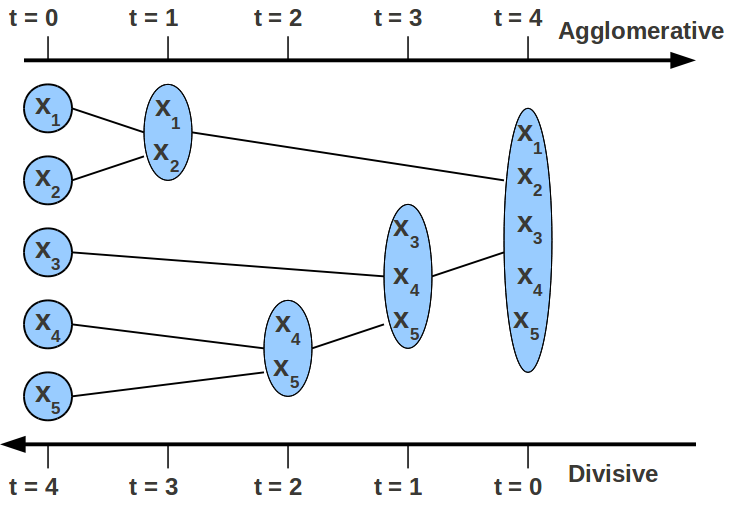
\includegraphics[width=0.6\textwidth]{hierarchical-clustering}
\caption{Etapas del agrupamiento jerárquico}
\label{fig:hier-clustering}
\end{figure}

\begin{figure}[htbp]
\centering
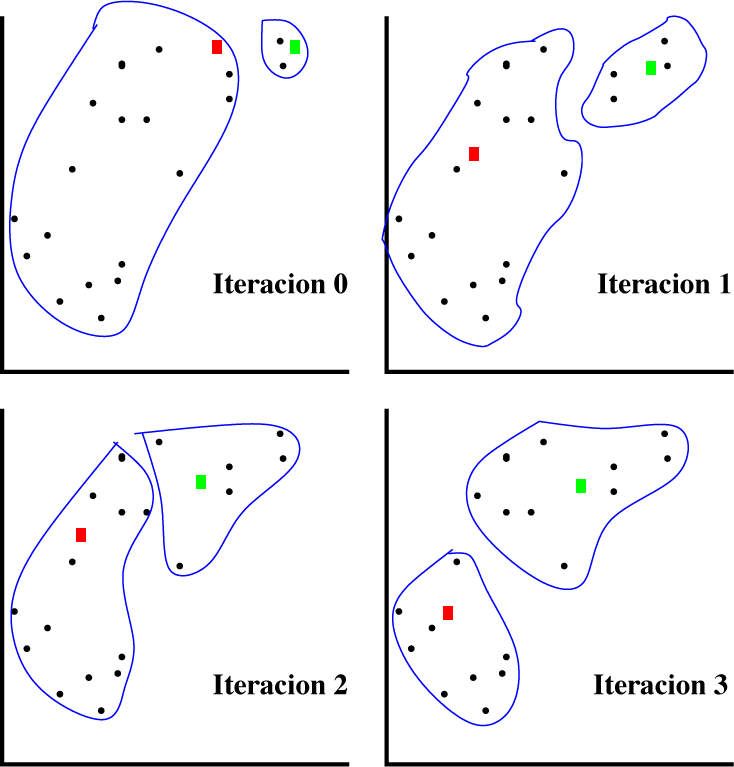
\includegraphics[width=0.6\textwidth]{k-medias}
\caption[Etapas del agrupamiento plano]{Etapas del agrupamiento plano \citep{RuizReina2013}}
\label{fig:k-medias}
\end{figure}

Además, uno de los retos de estos sistemas es cómo representar el conocimiento extraído en el entrenamiento para almacenarlo y usarlo posteriormente.

\section{Clasificadores}

Los clasificadores son programas que dado un documento de entrada, le asocia una categoría o etiqueta. Estos clasificadores han debido ser previamente entrenados mediante una técnica de aprendizaje automático, o bien programados con las reglas apropiadas.

En función del resultado de la clasificación, podemos distinguir dos tipos de clasificadores:
\nopagebreak
\begin{description}
\item[Clasificador binario] En este caso, existen dos posibles categorías a asocias a cada documento. Por ejemplo, un detector de \emph{spam} puede determinar que un mensaje de correo electrónico es spam o no lo es (es \emph{spam} o es \emph{ham}). El resultado puede venir --y es recomendable--, acompañado de un valor de confidencia (probabilidad de haber acertado).
\item[Clasificador múltiple] Aquí el documento puede asignarse a varias categorías, con un valor de confidencia diferente para cada una. Se podría después tener en cuenta solamente la categoría asignada con mayor probabilidad, o bien se infiere que pertenece simultáneamente a las $n$ categorías con mayor probabilidad.
\end{description}


\subsection{Bondad del clasificador (valor-F)}

Para la comparación de sistemas de búsqueda y recuperación de información disponemos de una métrica llamada valor-F\index{valor-F} (\emph{F-score}\index{F-score@\emph{F-score}}, \emph{F-measure}\index{F-measure@\emph{F-measure}} ó \emph{$F_1$ score}\index{F\_1 score@$F_1$ score}) siendo ésta la media armónica de otros dos indicadores \citep[Precisión y exhaustividad]{wikipedia-es}:
\begin{description}
\item[precisión \emph{(precision)}] \index{precisión}\index{precision@\emph{precision}}
Es la fracción de instancias recuperadas que son relevantes.
\begin{eqnarray}
\text{precisión} &=& \frac{|\{\text{relevantes}\}\cap\{\text{recuperados}\}|}{|\{\text{recuperados}\}|}
\end{eqnarray}
\item[exhaustividad \emph{(recall)}] \index{exhaustividad}\index{recall@\emph{recall}}
Es la fracción de instancias relevantes que han sido recuperadas.
\begin{eqnarray}
\text{exhaustividad} &=& \frac{|\{\text{relevantes}\}\cap\{\text{recuperados}\}|}{|\{\text{relevantes}\}|}
\end{eqnarray}
\item[valor-F \emph{(F-score)}] Media armónica de precisión y exhaustividad.
\begin{eqnarray}
F_1 &=& 2\times\frac{\text{precisión}\times\text{exhaustividad}}{\text{precisión}+\text{exhaustividad}}
\end{eqnarray}
\end{description}

Supongamos un clasificador binario:
\begin{itemize}
\item La medida de precisión será el porcentaje de documentos correctamente clasificados dentro del conjunto de prueba.
\item La medida de exhaustividad será el porcentaje de documentos del conjunto de referencia que han sido correctamente clasificados \citep{Perkins2010}.
\end{itemize}

\subsection{Resumen de procedimientos de preprocesamiento}

\begin{figure}[H]
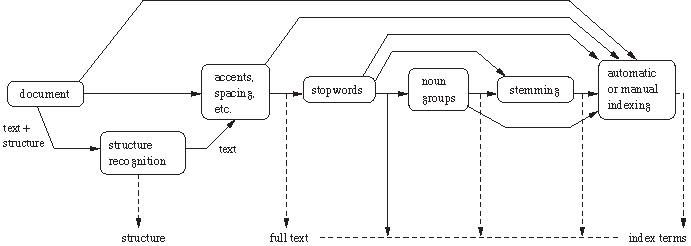
\includegraphics[width=0.98\textwidth]{procesamiento-textos-mod-ir}
\caption[Resumen de procedimientos de preprocesamiento]{Resumen de procedimientos de preprocesamiento \citep[ch. 7]{Baeza-Yates2011}}
\end{figure}

\section{Rendimiento en Python}

Se observó que la carga del modelo entrenado \path{GoogleNews-vectors-negative300.bin.gz} consumía mucho tiempo y espacio ($\approx$\si{4.5}{GiB} y unos 5 minutos). Este modelo ha sido publicado por Google en el repositorio del proyecto \codep{word2vec} basado en el \emph{dataset} de Google News (aproximadamente 100 mil millones de palabras). El modelo contiene vectores 300-dimensionales para 3 millones de palabras y de frases (bigramas y trigramas). Las frases se obtuvieron usando una aproximación dirigida por datos sencilla, como se encuentra descrito en \cite{DBLP:journals/corr/MikolovSCCD13}.

Por ello se convirtió inicialmente el modelo del \emph{Word2Vec} original en la representación interna provista por \codep{gensim}, que soporta en \emph{unpickling} de datos de NumPy, de mejor desempeño.

El procedimiento para la conversión es:

\begin{listing}[H]
\begin{minted}{python}
from gensim.models.word2vec import Word2Vec
# lectura sin optimizar
model_orig = Word2Vec.load_word2vec_format('GoogleNews-vectors-negative300.bin', binary=True)
# escritura optimizada
model_orig.save('GoogleNews-vectors-negative300.bin.gensim')
\end{minted}
\caption{Conversión del formato crudo \codep{word2vec} en el optimizado por \codep{gensim}}
\label{lst:word2vec-convert}
\end{listing}

Y para la carga de la versión optimizada:

\begin{listing}[H]
\begin{minted}{python}
from gensim.models.word2vec import Word2Vec
# lectura optimizada
model = Word2Vec.load('GoogleNews-vectors-negative300.bin.gensim', mmap='r')
\end{minted}
\caption{Lectura del modelo optimizado por \codep{gensim} previamente almacenado}
\label{lst:word2vec-convert}
\end{listing}


\cleardoubleevenemptypage
\part{Desarrollo del proyecto}
\label{part:desarrollo-proyecto}

%!TEX root = pfc-memoria.tex
%!TEX encoding = UTF-8 Unicode

%!TEX root = pfc-memoria.tex
%!TEX encoding = UTF-8 Unicode

\chapter{Análisis de requisitos}

\flushbottom


Este capítulo contiene la Especificación de Requisitos del Sistema (ERS en español, ó SRS del inglés \emph{System Requirements Specification})\index{ERS}\index{SRS} siguiendo las directrices de la norma IEEE~Std~830-1998 \citep{std830-1998} usando la notación de UML~2.5 \citep{UML2.5}

\section{Actores del sistema}

\SRSActor{title={Usuario},
label=usuario,
desc={Usuario normal de la aplicación, comúnmente un alumno en un puesto informático con la aplicación gráfica instalada, pantalla, procesador, teclado y ratón.},
comments={-/-},
stability=Alta}

\section{Objetivos}

\SRSObj{title={Biblioteca unificada de NLP y ML},
label=biblioteca-nlp-ml,
desc={Desarrollar una biblioteca unificada de NLP y ML para el análisis del sentimiento o polaridad de opiniones. La biblioteca debe proporcionar la funcionalidad necesaria para
\begin{enumerate}[a)]
\item procesar texto mediante diversos filtros (en la etapa de entrenamiento y la de clasificación),
\item aprender a clasificar el sentimiento automáticamente mediante algoritmos parametrizables de aprendizaje automático.
\end{enumerate}
Ambos grupos de funcionalidad deberán permitir la colaboración entre sí, en secuencia.},
comments={-/-},
stability=Alta}

\newpage
\SRSObj{title={GUI para el análisis de sentimiento},
label=gui,
desc={Desarrollar una aplicación de escritorio, con Interfaz Gráfica de Usuario multiplataforma, que haga uso del \refSRSObj{biblioteca-nlp-ml} para guiar al alumno en el análisis del sentimiento de opiniones sin necesidad de codificar nada.},
comments={-/-},
stability=Alta}


\section{Requisitos de información}

\SRSIrq{title={Fichero de configuración de sesión},
label=yaml,
desc={El sistema deberá proporcionar una manera de guardar y recuperar un fichero con la información necesaria para establecer la configuración de opciones de la sesión de trabajo actual con el programa.},
comments={Fichero de entrada y de salida.
Se recomienda un formato consumible por máquina y humano, sencillo, de tipo YAML.},
objasoc={\fullrefSRSObj{gui}},
reqasoc={-/-},
data={Datos de los parámetros ajustables presentes en los elementos del GUI:
\begin{itemize}
\item ruta a los ficheros de entrada,
\item opciones activas de preprocesamiento de texto,
\item opciones de la extracción de características,
\item parámetros establecidos en cada método de aprendizaje automático,
\item puntuaciones relativas obtenidas ($f$-values),
\item cualquier otro dato necesario para poder repetir el experimento y obtener los mismos resultados.
\end{itemize}},
priority=Media,
stability=Alta}

\newpage
\SRSIrq{title={Formato del fichero de entrenamiento},
label=traintsv,
desc={Es un fichero de texto plano, en formato TSV (tab-separated values), con línea de cabeceras y de cuatro columnas, sin adorno de los literales de cadena.},
comments={Fichero de entrada. El detalle de los formatos de fichero se encuentra en \url{https://www.kaggle.com/c/sentiment-analysis-on-movie-reviews/data}},
objasoc={\fullrefSRSObj{gui}},
reqasoc={-/-},
data={Las columnas son: \begin{enumerate}
\item PhraseId (numérico y único)
\item SentenceId (numérico)
\item Phrase (cadena con el texto)
\item Sentiment (numérico).
\end{enumerate}
La clasificación del sentimiento corresponde de la siguiente manera:
\begin{eqnarray*}
0 & \longrightarrow & \text{negativo} \\
1 & \longrightarrow & \text{algo negativo} \\
2 & \longrightarrow & \text{neutro} \\
3 & \longrightarrow & \text{algo positivo} \\
4 & \longrightarrow & \text{positivo}
\end{eqnarray*}},
priority=Alta,
stability=Alta}

\SRSIrq{title={Formato del fichero de evaluación},
label=testtsv,
desc={Es un fichero de texto plano, en formato TSV (tab-separated values), con línea de cabeceras y de tres columnas, sin adorno de los literales de cadena.},
comments={Fichero de entrada. El detalle de los formatos de fichero se encuentra en \url{https://www.kaggle.com/c/sentiment-analysis-on-movie-reviews/data}},
objasoc={\fullrefSRSObj{gui}},
reqasoc={\fullrefSRSIrq{traintsv}},
data={Análogo al \refSRSIrq{traintsv}, pero sin la última columna del sentimiento.},
priority=Alta,
stability=Alta}

\newpage
\SRSIrq{title={Formato del fichero de envío},
label=submissioncsv,
desc={Es un fichero de texto plano, en formato CSV (comma-separated values), con línea de cabeceras y de dos columnas},
comments={Fichero de salida. El detalle de los formatos de fichero se encuentra en \url{https://www.kaggle.com/c/sentiment-analysis-on-movie-reviews/data}},
objasoc={\fullrefSRSObj{gui}},
reqasoc={\fullrefSRSIrq{traintsv}},
data={Las columnas son: \begin{enumerate}
\item PhraseId (numérico y único)
\item Sentiment (numérico). Análoga correspondencia que en \refSRSIrq{traintsv}.
\end{enumerate}},
priority=Media,
stability=Alta}


\section{Requisitos funcionales}

\SRSUc{title={Cargar fichero de entrenamiento},
label={loadtraintsv},
desc={Mediante esta función, el usuario cargará un fichero de entrenamiento (\path{train.tsv}).},
precond={-/-},
steps={\begin{enumerate}
\item El usuario solicita cargar un nuevo fichero de entrenamiento.
\item El sistema ofrece un cuadro de diálogo para que el usuario seleccione el fichero.
\item El usuario selecciona el fichero.
\item El sistema ofrece la posibilidad de cargar sólo un número concreto de las primeras líneas.
\item El usuario escoge si se carga sólo un número concreto de las primeras líneas, o todas las del fichero.
\item El sistema lee el fichero a memoria y muestra el contenido del mismo en la tabla de resultados.
\end{enumerate}},
postcond={\begin{enumerate}
\item Se asocia en el diccionario de configuración la ruta al fichero de entrenamiento y la opción de carga parcial de las primeras líneas.
\item El contenido del fichero se encuentra visible de forma tabulada en la tabla de datos.
\end{enumerate}},
exceptions={Si el formato de fichero no concuerda con el especificado en \refSRSIrq{traintsv}, se produce un error.},
comments={-/-},
objasoc={\fullrefSRSObj{gui}},
reqasoc={\fullrefSRSIrq{traintsv}},
priority=Alta,
stability=Alta}

\begin{landscape}
\begin{figure}[htbp]
\centering
\resizebox{!}{0.76\textwidth}{\input{use-cases.puml}}
\caption{Diagrama de casos de uso}
\label{fig:uml-uc}
\end{figure}
\end{landscape}

%\begin{figure}[htbp]
%\centering
%\resizebox{0.6\textwidth}{!}{\input{use-cases-es.puml}}
%\caption{Diagrama de casos de uso (E/S)}
%\label{fig:uml-uc-es}
%\end{figure}
%
%\begin{figure}[htbp]
%\centering
%\resizebox{0.6\textwidth}{!}{\input{use-cases-sentanal.puml}}
%\caption{Diagrama de casos de uso (Análisis del senimiento)}
%\label{fig:uml-uc-sentanal}
%\end{figure}

\section{Requisitos no funcionales}

\SRSNfr{title={Multiplataforma},
label=multiplataforma,
desc={La aplicación será multiplataforma, al menos para los sistemas Mac~OS~X, Windows y GNU/Linux.},
comments={La estética del GUI no es determinante.},
objasoc={\fullrefSRSObj{gui}},
reqasoc={-/-},
priority=Alta,
stability=Alta}

\SRSNfr{title={Con visualización de la tabla de datos},
label=tabla-datos,
desc={En la medida de lo posible, debe verse una tabla de datos para examinar cómo se van aplicando las sucesivas transformaciones.},
comments={Es para promover el uso didáctico de la aplicación.},
objasoc={\fullrefSRSObj{gui}},
reqasoc={-/-},
priority=Media,
stability=Alta}

\SRSNfr{title={Con visualización del progreso},
label=progreso,
desc={En la medida de lo posible, debe verse una indicación del progreso en cada función que se realice sobre los datos.},
comments={Es para no dar la impresión al usuario de que la aplicación se haya bloqueado, al tratar con tablas de datos grandes.},
objasoc={\fullrefSRSObj{gui}},
reqasoc={-/-},
priority=Media,
stability=Alta}

\raggedbottom



%!TEX root = pfc-memoria.tex
%!TEX encoding = UTF-8 Unicode

\chapter{Diseño de la solución}

\epigraph{``La función de un buen software es hacer que lo complejo aparente ser simple.''}{\textsc{Grady Booch} (1955--)}

En este capítulo comentamos las decisiones de diseño tomadas para la construcción de la aplicación teniendo en cuenta la ERS del \fullref{chap:analisis-requisitos}.

\section{Patrón de diseño}

Como la aplicación será una aplicación de escritorio, con su interfaz gráfica de usuario (GUI), diseñaremos el sistema de manera adecuada para dar soporte a un desarrollo rápido de la aplicación dirigida por eventos \emph{(Event-driven programming).}\index{EDP}\index{Event-driven programming@\emph{Event-driven programming}}

Se diseñará un sistema basado en el patrón Modelo-Vista-Presentador (MVP, \emph{Model-View-Presenter} en inglés)\index{MVP}\index{Modelo-Vista-Presentador}\index{Model-View-Presenter@\emph{Model-View-Presenter}}. Es un patrón parecido al conocido Modelo-Vista-Controlador (MVC, \emph{Model-View-Controller} en inglés)\index{MVC}\index{Modelo-Vista-Controlador}\index{Model-View-Controller@\emph{Model-View-Controller}}, sin embargo presenta algunas diferencias que cabe destacar (véase \autoref{fig:MVP-MVC}):

\begin{itemize}
\item En el MVP, el Controlador pasa a llamarse Presentador, y se define como un Controlador-supervisor, colocándose como hombre-en-el-medio (mitm, \emph{man-in-the-middle})\index{mitm}\index{man-in-the-middle@\emph{man-in-the-middle}} entre la Vista y el Modelo.
\item Así, el Modelo no puede interactuar con la Vista de manera directa, sino sólo a través del Presentador.
\item Esto permite mayor independencia de código y mayores oportunidades de reutilización, al ser más sencillo cambiar la Vista por otra sin afectar al Modelo, que contiene el acceso a la información y la lógica de negocio.
\end{itemize}

\begin{figure}[htbp]\centering
\begin{subfigure}[b]{0.49\textwidth}\centering
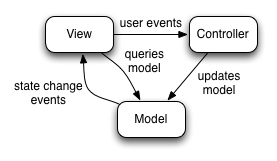
\includegraphics[width=0.85\textwidth]{MVC}
\caption{Modelo-Vista-Controlador (MVC)}
\end{subfigure}
\begin{subfigure}[b]{0.49\textwidth}\centering
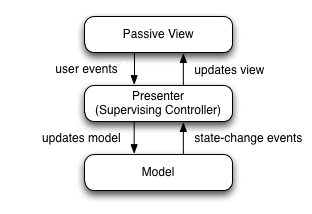
\includegraphics[width=0.94\textwidth]{MVP}
\caption{Modelo-Vista-Presentador (MVP)}
\end{subfigure}
\caption[Patrones MVC y MVP]{Patrones MVC y MVP. La principal diferencia en MVP es que el Modelo no puede interactuar con la Vista si no es a través del Presentador. \\
{\footnotesize \url{http://www.gwtproject.org/articles/testing_methodologies_using_gwt.html}}}
\label{fig:MVP-MVC}
\end{figure}

\section{Arquitectura del sistema}

La aplicación se desarrolla usando el lenguaje de programación Python~3.

En la \fullref{fig:architecture} se encuentra un resumen visual de la situación de cada componente dentro del patrón MVP y la colaboración entre ellos.

Los componentes (todos de software libre) que se reutilizan son:
\begin{description}
\item[Qt5]\index{Qt} Biblioteca de herramientas gráficas para la creación de interfaces de usuario ---con licencia de software libre--- en C++ que proporciona widgets y un framework de desarrollo de GUI compatible con la programación dirigida por eventos, soportado por las plataformas Windows, GNU/Linux y Mac~OS~X, entre otros \citep{Huang2015}. Actualmente mantenido por Digia.
\item[PyQt5] Puente \emph{(binding)} entre Python~2/3 y la biblioteca Qt5, mantenido por Riverbank Computing \citep{Summerfield2008}.
\item[QML] \emph{Qt Markup Language}\index{QML} es un motor declarativo de interfaces de usuario para Qt con sintaxis compatible con ECMAScript, integrado dentro de las versiones modernas de Qt5 \citep{web:QmlBook}.
\item[NLTK3] \emph{Natural Language Toolkit}\index{NLKT} es una biblioteca de utilidades en procesamiento de texto para Python \citep{Perkins2014}.
\item[scikit-learn] Biblioteca en Python para aprendizaje automático \citep{Pedregosa2011}.
\item[NumPy] Biblioteca en Python/C++ para el tratamiento de vectores/matrices numéricos y precisión arbitraria de manera eficiente desde Python \citep{Bressert2012}.
\end{description}

Los componentes a desarrollar son dos módulos en Python, uno para cubrir el \fullrefSRSObj{gui}, y el segundo módulo para el \fullrefSRSObj{biblioteca-nlp-ml}; y que se describen a continuación:
\begin{description}
\item[\codep{pfcsamr.gui}] Implementa el Presentador que recibe y maneja los eventos generados por el usuario al interactuar en el GUI, y canaliza las operaciones comandadas hacia el Modelo. Así mismo, monitoriza los cambios que se produzcan en el Modelo y refleja estos cambios en el GUI actualizando el estado de la pantalla. Este modelo incluye también la descripción de la interfaz en el lenguaje declarativo QML.\index{QML}
\item[\codep{pfcsamr.orchestrator}] Implementa el Modelo que actúa «orquestando» todo el proceso de análisis de sentimiento, coordinando de manera coherente los paquetes de NLTK3 y scikit-learn, y ofreciendo toda la funcionalidad de E/S.
\end{description}

Los componentes a desarrollar se indican en color verde en la \autoref{fig:architecture}, mientras el resto son componentes proporcionados por proyectos de software libre disponibles públicamente.

\begin{figure}[htbp]
\centering
\vspace{0.5cm}
\resizebox{0.75\textwidth}{!}{\input{architecture.puml.tex}}
\caption{Diagrama de arquitectura de componentes}
\label{fig:architecture}
\end{figure}

\section{Interfaz de usuario}

A continuación se muestran los bocetos de las pantallas a crear.

\subsection{Elementos comunes}

La pantalla principal es una ventana formada por 5 pestañas que guían al alumno a lo largo de las etapas de una tarea de análisis de sentimiento, y en la parte inferior una tabla de los datos obtenidos en cada etapa (\autoref{fig:gui-1-load}).

Todas las pantallas comparten los siguientes elementos:
\begin{enumerate}
\item Barra de menú, con las siguientes opciones:
\begin{enumerate}
\item \menu{File > New} (atajo de teclado: \keys{\cmd+N})\\
Pulsando esta opción se reestablece toda la configuración con los valores por defecto para iniciar una nueva sesión con un documento nuevo.
\item \menu{File > Open...} (atajo de teclado: \keys{\cmd+O})\\
Pulsando esta opción se puede abrir un fichero \path{project.yaml} del que leer el diccionario de configuración de la sesión, y se actualiza la sesión con la información leída. Véase \fullrefSRSUc{loadyaml}.
\item \menu{File > Save...} (atajo de teclado: \keys{\cmd+S})\\
Pulsando esta opción se guarda un fichero \path{project.yaml} con el diccionario de la configuración de la sesión en curso. Véase \fullrefSRSUc{saveyaml}.
\item \menu{File > Quit} (atajo de teclado: \keys{\cmd+Q})\\
Cierra la aplicación.
\end{enumerate}
\item Mitad superior con las pestañas ordenadas para guiar en el proceso: Load, Preprocess, Features, Learn y Classify, y el panel de configuración de opciones de cada etapa.
\item Mitad inferior con la tabla de datos de resultados de cada operación, en columnas y filas con controles de desplazamiento horizontal y vertical.
\item Barra de estado con tres elementos:
\begin{enumerate}
\item Texto descriptivo para mostrar qué se está haciendo o qué operación se ha terminado.
\item Barra de progreso de la operación.
\item Contador de la iteración actual de la operación en curso. Se incrementa en pasos de 32 en 32 filas para no penalizar el rendimiento con actualizaciones constantes.
\end{enumerate}
\end{enumerate}

\FloatBarrier
\newpage
\subsection{Pestaña LOAD}

La primera pestaña, \nombrebf{LOAD} sirve para cargar el fichero de entrenamiento \path{train.tsv} (\autoref{fig:gui-1-load}).

Contiene los siguientes elementos:
\begin{enumerate}
\item Botón para desplegar el selector de fichero.
\item Etiqueta de texto para visualizar la ruta al fichero.
\item Casilla de verificación para habilitar la carga parcial.
\item Selector numérico del número de primeras líneas de la carga parcial.
\item Botón de carga.
\end{enumerate}

La funcionalidad de los elementos siguen la especificación del \fullrefSRSUc{loadtraintsv}.

\begin{figure}[htbp]
\centering
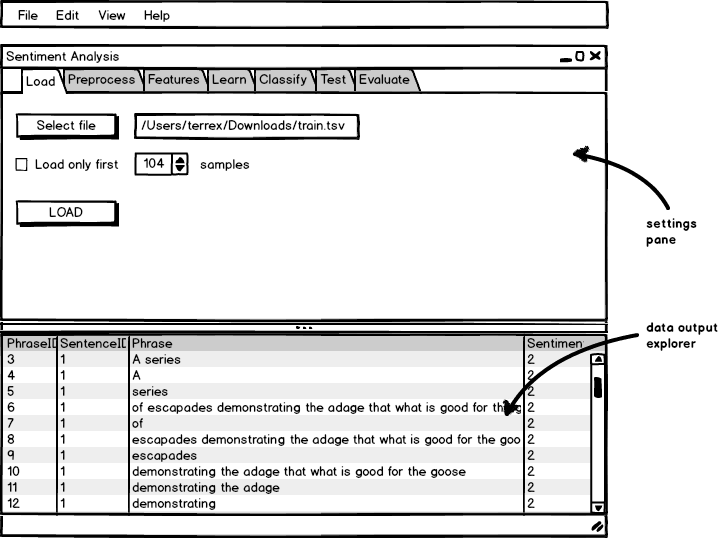
\includegraphics[width=14cm]{gui-1-load}
\caption{Wireframe pestaña LOAD}
\label{fig:gui-1-load}
\end{figure}

\FloatBarrier
\newpage
\subsection{Pestaña PREPROCESS}

La segunda pestaña, \nombrebf{PREPROCESS} sirve para preprocesar el texto de los documentos de entrenamiento aplicando los filtros y transformaciones indicados (\autoref{fig:gui-2-preprocess}).

Contiene los siguientes elementos:
\begin{enumerate}
\item Casilla de verificación para volver a unir las contracciones separadas.
\item Casilla de verificación para expandir las contracciones en sus palabras equivalentes sin contracción. Véase \autoref{subsec:tokenizacion}.
\item Casilla de verificación para suprimir palabras vacías (\emph{stopwords}, véase \autoref{subsec:stopwords}).
\item Casilla de verificación para habilitar el reemplazo de palabras, con una de las dos opciones excluyentes siguientes:
\begin{enumerate}
\item Radicar (\emph{stemming}, \autoref{subsec:stemming}).
\item Lematizar (\autoref{subsec:lematizacion}).
\end{enumerate}
\item Casilla de verificación para anotar la parte-de-la-oración. Véase \autoref{subsec:postagging}.
\item Botón de RUN para ejecutar la etapa.
\end{enumerate}

La funcionalidad de los elementos siguen la especificación del \fullrefSRSUc{preproc}.

\begin{figure}[htbp]
\centering
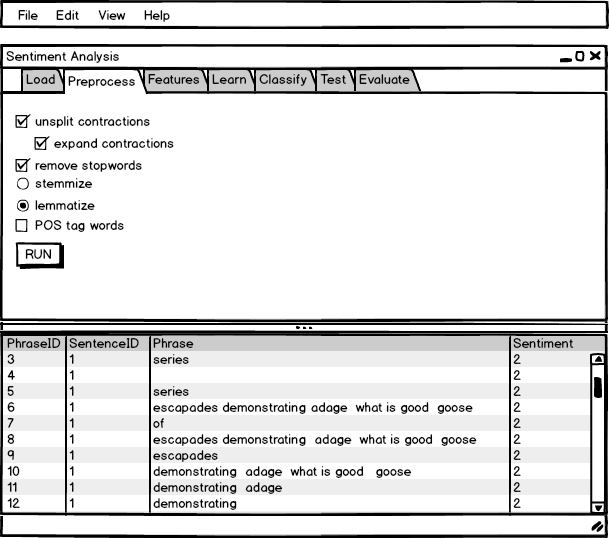
\includegraphics[width=12cm,clip=true,trim=0 0 0 38pt]{gui-2-preprocess}
\caption{Wireframe pestaña PREPROCESS}
\label{fig:gui-2-preprocess}
\end{figure}

\FloatBarrier
\newpage
\subsection{Pestaña FEATURES}

\todo{por aki}

\begin{figure}[htbp]
\centering
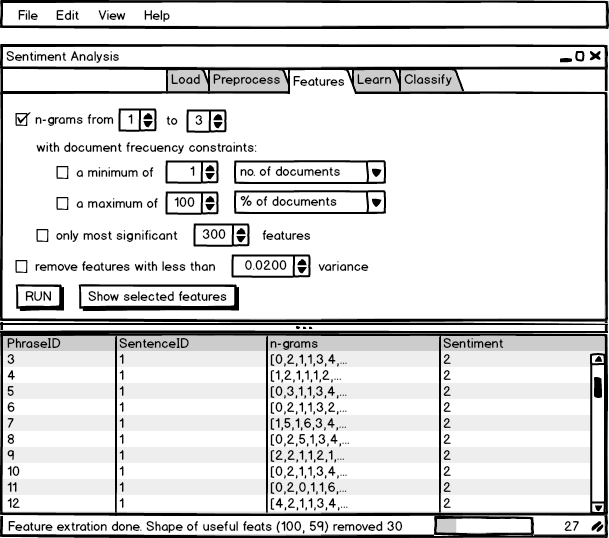
\includegraphics[width=12cm,clip=true,trim=0 0 0 38pt]{gui-3-features}
\caption{Wireframe pestaña FEATURES}
\label{fig:gui-3-features}
\end{figure}

\FloatBarrier
\newpage
\subsection{Pestaña LEARN}

\begin{figure}[htbp]
\centering
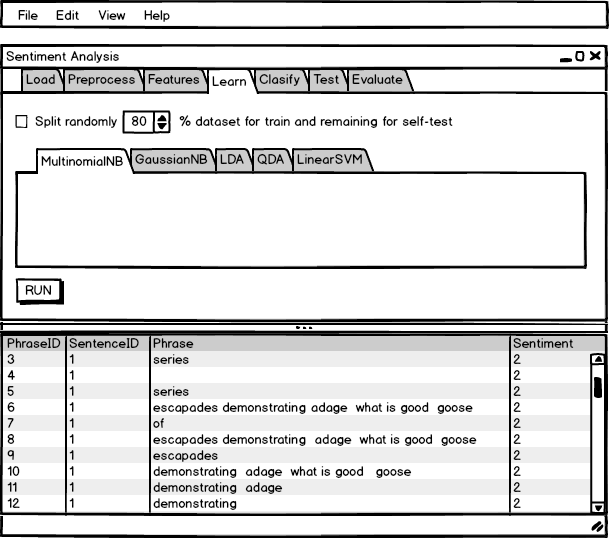
\includegraphics[width=12cm,clip=true,trim=0 0 0 38pt]{gui-4-learn}
\caption{Wireframe pestaña LEARN}
\label{fig:gui-4-learn}
\end{figure}

\FloatBarrier
\newpage
\subsection{Pestaña CLASSIFY}

\begin{figure}[htbp]
\centering
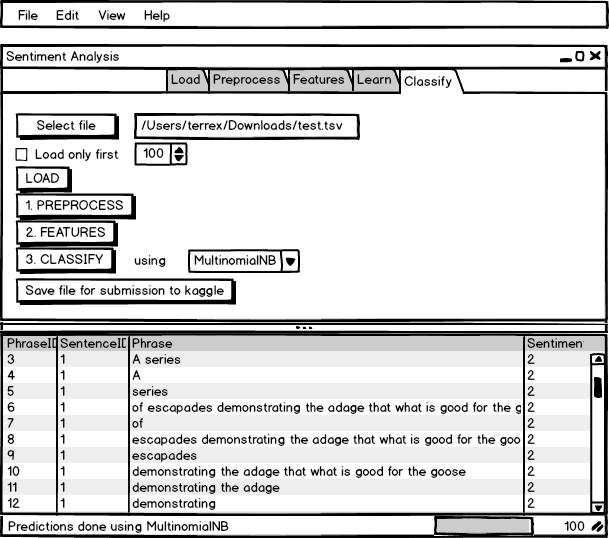
\includegraphics[width=12cm,clip=true,trim=0 0 0 38pt]{gui-5-classify}
\caption{Wireframe pestaña CLASSIFY}
\label{fig:gui-5-classify}
\end{figure}


\section{Clases}

A continuación se describen las clases principales necesarias.

\subsection{\codep{pfcsamr.gui.MainPfcsamrApp}}

\subsection{\codep{pfcsamr.orchestrator.Orchestrator}}

\subsection{\codep{pfcsamr.orchestrator.MyTableModel}}


\begin{landscape}
\begin{figure}[htbp]
\centering
\resizebox{!}{0.99\textwidth}{\input{classes.puml.tex}}
\caption{Diagrama de clases}
\label{fig:classes}
\end{figure}
\end{landscape}



\section{Secuencias}




\resizebox{0.5\textwidth}{!}{\input{diag1.puml.tex}}

\ldots

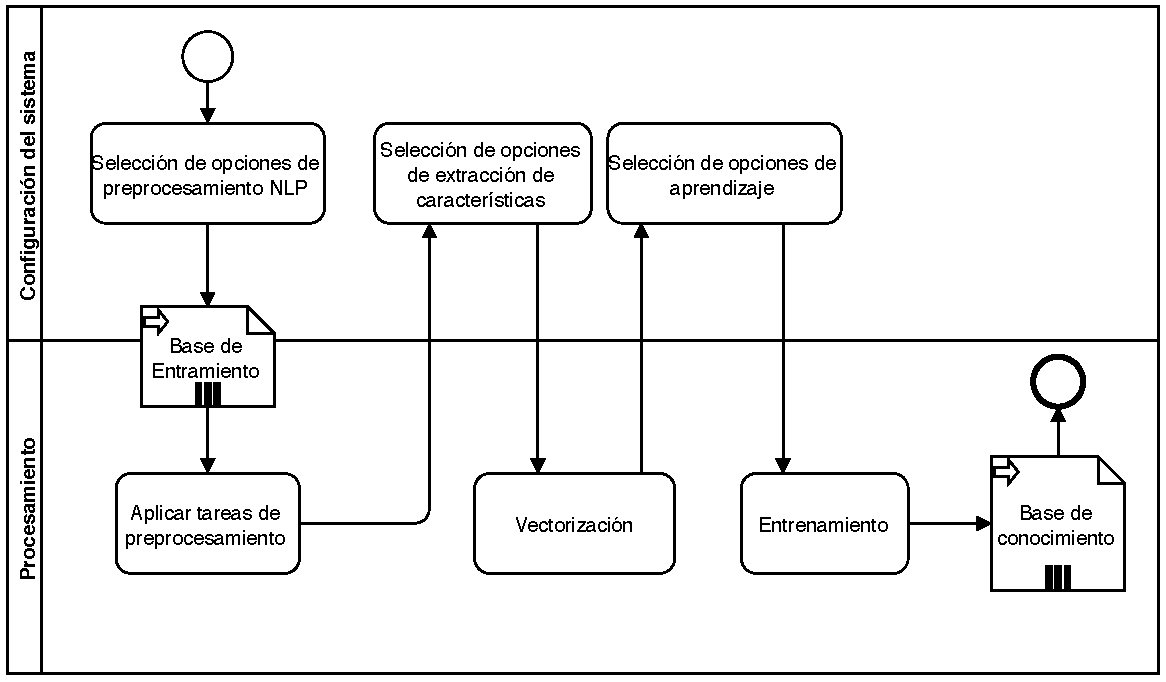
\includegraphics[width=\textwidth]{bpmn-entrenamiento}

\ldots

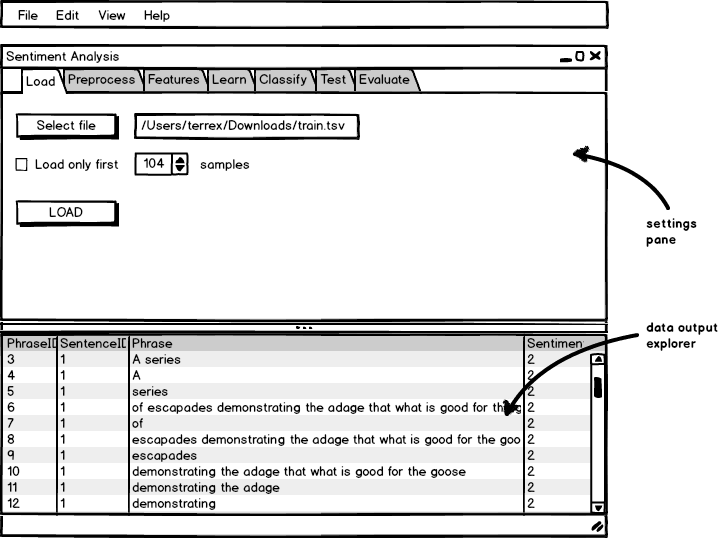
\includegraphics[width=14cm]{gui-1-load}

\ldots

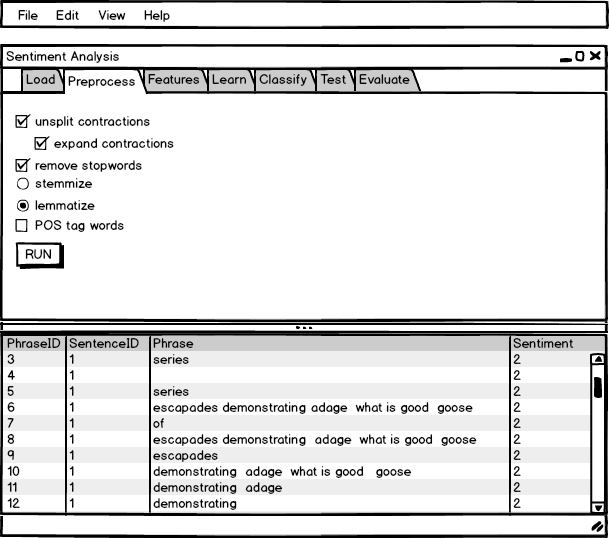
\includegraphics[width=12cm]{gui-2-preprocess}

\ldots

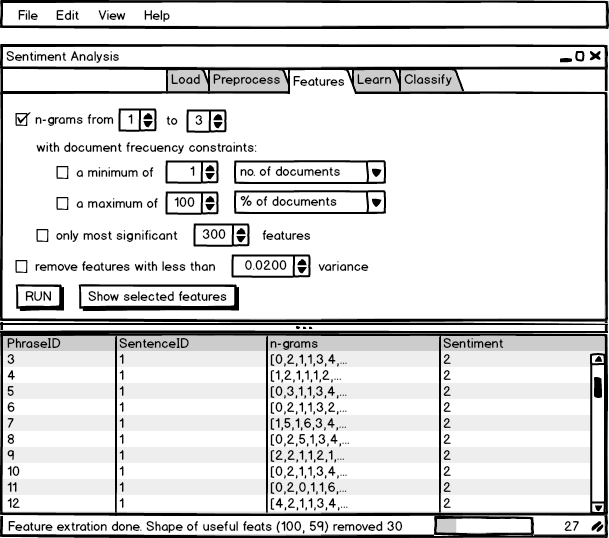
\includegraphics[width=12cm]{gui-3-features}

\ldots

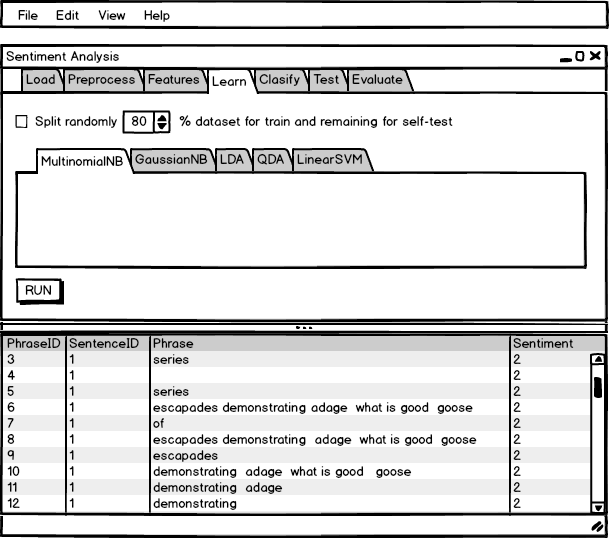
\includegraphics[width=12cm]{gui-4-learn}

\ldots

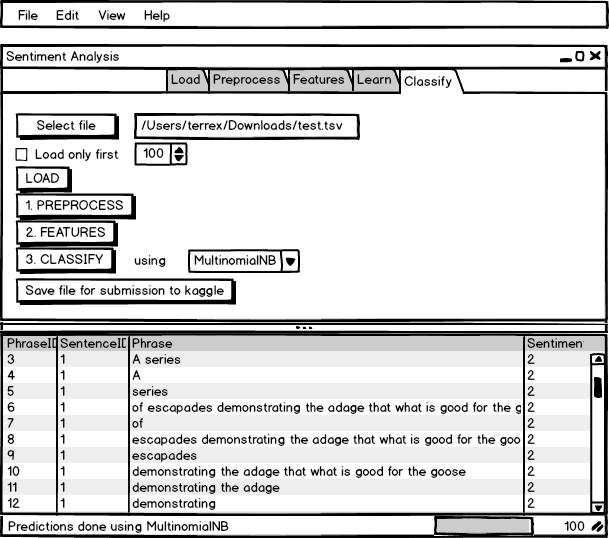
\includegraphics[width=12cm]{gui-5-classify}

\ldots


%!TEX root = pfc-memoria.tex
%!TEX encoding = UTF-8 Unicode

\chapter{Implementación}
\label{chap:implementacion}

\epigraph{``La mejor forma de predecir el futuro es implementarlo.''}{\textsc{David Heinemeier Hansson} (1979--)}

La implementación se encuentra en los ficheros del CD-ROM adjunto. En este capítulo describimos algunos aspectos notables de la implementación, y lecciones aprendidas durante el desarrollo.

\section{Lenguajes declarativos de descripción de interfaces de usuario}

Teniendo en cuenta los requisitos \fullrefSRSObj{gui} y \fullrefSRSNfr{multiplataforma}, y mi poca experiencia reciente en aplicaciones de escritorio con GUI, opté por usar un framework de desarrollo con descripción declarativa del GUI. Para la construcción de interfaces de usuario existen dos enfoques, principalmente:
\begin{itemize}
\item De manera \nombrebf{imperativa}, invocando desde código del lenguaje de programación a las clases y métodos que proporcione el framework de desarrollo para colocar los elementos en la pantalla.
\item Otra manera más independiente \nombrebf{declarativa}, sin programación, con la descripción del árbol o un conjunto de elementos por nombre y atributos que el motor que proporcione el framework interpreta y convierte en las llamadas análogas del caso imperativo.
\end{itemize}

El enfoque declarativo tiene como ventaja principal la independencia entre aspectos de la visualización y del código; facilitando que personas con perfiles distintos (diseñador, y programador) se puedan dedicar a cada parte del desarrollo sin necesidad de tener demasiados conocimientos del otro aspecto. Tradicionalmente, se han usado sublenguajes de XML para este propósito \citep{Hurtado2004}.

\subsection{Kivy}

Durante el período de investigación de los frameworks existentes, probé inicialmente Kivy.\footnote{\url{http://kivy.org/}}

Kivy es un framework de desarollo multiplataforma e independiente del dispositivo. Se utiliza OpenGL para renderizar la pantalla y los elementos, sin utilizar las bibliotecas nativas de las plataformas destino, lo que lo hace muy independiente del entorno de ejecución (puede ser Windows, GNU/Linux, Android, iOS, XBOX, \ldots), y además la visualización es idéntica en todos ellos. Se orienta sobretodo en el desarrollo de videojuegos y de interfaces para dispositivos multitáctiles.

El lenguaje de descripción de interfaces en Kivy se denomina KV Language y es de tipo YAML. Es un documento, generalmente con extensión \path{.kv}, directamente usable desde Python con el árbol de elementos de interfaz: rejillas de layouts, disposición en columnas o filas, etiquetas, cuadros de entrada de texto, botones, \ldots, ordenados de forma jerárquica en el árbol cuyo padre contiene a los elementos del interior de su área o rectángulo ``canvas'' de dibujo (\autoref{fig:kv-lang}).\index{canvas@\emph{canvas}}

\begin{figure}[htbp]
\centering
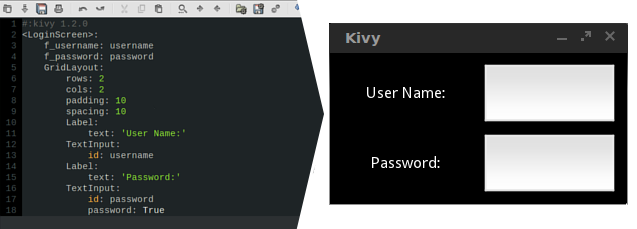
\includegraphics[width=0.99\textwidth]{kv-lang}
{\footnotesize\url{http://kivy.org/docs/gettingstarted/rules.html}}
\caption{KV Language para descripción de interfaces en Kivy}
\label{fig:kv-lang}
\end{figure}

Kivy~1.9 en aquel momento estaba en fase beta, y soportaba parcialmente Python~3. Sin embargo, sí funcionaba perfectamente para Python~2. No obstante, es de todos conocido los problemas de compatibilidad entre Python~3 y 2, y preferí usar el más reciente, Python~3, para el código del proyecto, por asegurar la aplicabilidad futura del proyecto. Hice algunas modificaciones en el núcleo de Kivy para modernizarlo,\footnote{Mis contribuciones al proyecto se pueden consultar en \url{https://github.com/kivy/kivy/pulls?q=is:pr+author:terrex+is:closed}} pero me estaba acumulando mucho retraso y lo abandoné en favor del lenguaje declarativo proporcionado por Qt conocido como QML.

\FloatBarrier
\newpage
\subsection{QML (Qt)}

Por contrapartida, las bibliotecas de Qt están bastante maduras. Se usan en el escritorio KDE desde siempre, y ha pasado a estar bajo el control de diferentes compañías ---Trolltech, Nokia, Digia---, que ofrecían diferentes licencias de uso, algo que siempre ha traído polémica en la comunidad de software libre alrededor de GNU/Linux.\footnote{\url{https://en.wikipedia.org/wiki/Qt_(software)\#Licensing}}
No obstante en los últimos años se han liberado versiones con licencias completamente compatibles con la definición de software libre de la \emph{Free Software Foundation}~(FSF).\index{FSF}

Qt también es multiplataforma, pero además ofrece una apariencia más integrada con el resto de la plataforma, ya que hace uso de las bibliotecas nativas para el renderizado de los elementos, sin tener un impacto visual reconocible dentro del ecosistema del sistema operativo (\autoref{fig:qt-multiplatform}).


\begin{figure}[htbp]
\centering
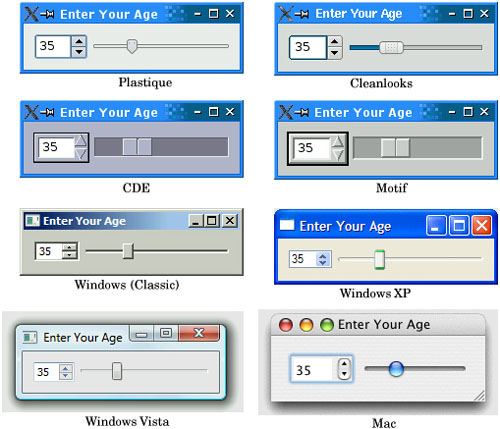
\includegraphics[width=0.7\textwidth]{qt-multiplatform}
{\footnotesize\url{http://www.veryhman.com/qt/ch01lev1sec3.html}}
\caption{Misma aplicación Qt en distintos entornos}
\label{fig:qt-multiplatform}
\end{figure}

A partir de la versión Qt~4.8, el framework incorpora el módulo QtQuick, que es el intérprete del lenguaje QML (acrónimo del inglés \emph{Qt Modeling Language})\index{QML}. Está basado en JavaScript, de manera que es muy similar al lenguaje KV de Kivy pero con más llaves \verb={}=, sólo que se permite toda la funcionalidad e interactividad que se pueda incorporar a través de JavaScript (ECMAScript). El documento base es una estructura en JSON (del inglés \emph{JavaScript Object Notation})\index{JSON} con la descripción de la interfaz en forma de árbol jerárquico.

Además, el framework ofrece su propio IDE llamado Qt~Creator, incluyendo un editor con reconocimiento de la sintaxis del lenguaje QML, algo que se agradece mucho.

Se puede ver un extracto del código QML en el \autoref{lst:qml-extract} que ha sido necesario para generar la pantalla de la \autoref{fig:qml-extract}. El problema principal con QML es la calidad de la documentación. Está desactualizada, y además se necesita mayor soporte de los elementos existentes en Qt para su uso desde QML.

\begin{figure}[htbp]
\centering
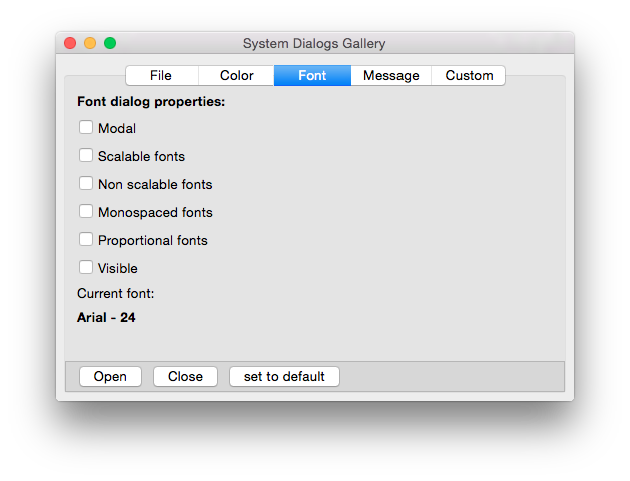
\includegraphics[width=0.8\textwidth,trim=56pt 80pt 56pt 30pt,clip]{qml-extract}
\caption{Aplicación de muestra de QtQuick (QML)}
\label{fig:qml-extract}
\end{figure}


\begin{listing}[phtb]
\begin{minted}[fontsize=\small]{js}
import QtQuick 2.2
import QtQuick.Controls 1.2

ApplicationWindow {
    title: "System Dialogs Gallery"
    width: 580
    height: 480

    TabView {
        /*...*/
        Tab {
            Column {
                id: optionsColumn
                anchors.fill: parent
                anchors.margins: 12
                spacing: 8
                Label {
                    font.bold: true
                    text: "Font dialog properties:"
                }
                CheckBox {
                    id: fontDialogModal
                    text: "Modal"
                    checked: true
                    Binding on checked { value: fontDialog.modality != Qt.NonModal }
                }
                CheckBox {
                    id: fontDialogScalableFonts
                    text: "Scalable fonts"
                    Binding on checked { value: fontDialog.scalableFonts }
                }
                /* ... */
                Label {
                    text: "Current font:"
                }
                Label {
                    id: fontLabel
                    text: "<b>" + fontDialog.font.family + " - " + fontDialog.font.pointSize + "</b>"
                    MouseArea {
                        anchors.fill: parent
                        onClicked: fontDialog.open()
                    }
                }
            }            
        }
        /*...*/
    }
}
\end{minted}
\caption{Extracto del QML de la aplicación de muestra}
\label{lst:qml-extract}
\end{listing}


El mayor problema que tuve fue la implementación de la tabla de datos. Según se extrae de la documentación, en QML existe el elemento \codep{TableView}, que debe incluir un \codep{TableViewColumn} para cada columna, clase que no tiene correspondencia en el Qt imperativo. Además, los datos deben ser provistos por filas, y una vez seleccionada la fila, tomar el dato de la columna necesaria; no permitiendo una matriz de filas y columnas de manera directa y accedido por la coordenada de la celda. Por eso es necesario reimplementar (\autoref{lst:MyTableModel}) un objeto con la interfaz \codep{QAbstractTableModel} y asignárselo vía Python en lugar de vía QML como cabría esperarse. No obstante una vez comprendido cómo se exportan los elementos de Qt a QML, se observa que es muy flexible, y que en el futuro, con un poco más de desarrollo, será QML completamente funcional y una alternativa real a la descripción imperativa de la interfaz.

\begin{listing}[htbp]
\begin{minted}{python}
from PyQt5.QtCore import QAbstractTableModel, QVariant, pyqtSlot, QModelIndex
import numpy as np

class MyTableModel(QAbstractTableModel):
    def __init__(self, headings, data):
        super().__init__()
        self.my_headings = headings
        if not hasattr(data, 'shape'):
            data = np.array(data)
        self.my_data = data

    @pyqtSlot(QModelIndex, result=int)
    @pyqtSlot(result=int)
    def rowCount(self, QModelIndex_parent=None, *args, **kwargs):
        return self.my_data.shape[0]

    @pyqtSlot(QModelIndex, result=int)
    @pyqtSlot(result=int)
    def columnCount(self, QModelIndex_parent=None, *args, **kwargs):
        return self.my_data.shape[1]

    @pyqtSlot(QModelIndex, int, result=QVariant)
    @pyqtSlot(QModelIndex, result=QVariant)
    def data(self, index: QModelIndex, role: int=None) -> QVariant:
        return str(self.my_data[index.row(), role - 32])

    @pyqtSlot(int, int, int, result=str)
    @pyqtSlot(int, int, result=str)
    def headerData(self, section: int, orientation: int, role: int=None):
        return self.my_headings[section]

    def roleNames(self):
        # los 32 primeros ``roles'' están reservados a Qt
        # para los roles personalizados, tenemos que empezar en el 32
        return dict(enumerate(self.my_headings, 32))
\end{minted}
\caption{Implementación de \codep{MyTableModel}}
\label{lst:MyTableModel}
\end{listing}

No obstante la complejidad del paquete QtQuick es bastante alta, y la potencia descriptiva de QML también. Tanto que la mayoría de los elementos de QML están implementados a su vez en el propio lenguaje QML, lo que denota una expresividad suficientemente versátil (\autoref{lst:qml-checkbox}).

\begin{listing}[phtb]
\begin{minted}[fontsize=\small]{js}
import QtQuick 2.2
import QtQuick.Controls 1.2
import QtQuick.Controls.Private 1.0
AbstractCheckable {
    id: checkBox
    property int checkedState: checked ? Qt.Checked : Qt.Unchecked
    property bool partiallyCheckedEnabled: false
    property bool __ignoreChecked: false
    property bool __ignoreCheckedState: false
    style: Qt.createComponent(Settings.style + "/CheckBoxStyle.qml", checkBox)
    activeFocusOnTab: true
    Accessible.role: Accessible.CheckBox
    Accessible.name: text
    __cycleStatesHandler: __cycleCheckBoxStates
    onCheckedChanged: {
        if (!__ignoreChecked) {
            __ignoreCheckedState = true;
            checkedState = checked ? Qt.Checked : Qt.Unchecked;
            __ignoreCheckedState = false;
        }
    }
    onCheckedStateChanged: {
        __ignoreChecked = true;
        if (checkedState === Qt.PartiallyChecked) {
            partiallyCheckedEnabled = true;
            checked = false;
        } else if (!__ignoreCheckedState) {
            checked = checkedState === Qt.Checked;
        }
        __ignoreChecked = false;
    }
    onPartiallyCheckedEnabledChanged: {
        if (exclusiveGroup && partiallyCheckedEnabled) {
            console.warn("Cannot have partially checked boxes in an ExclusiveGroup.");
        }
    }
    onExclusiveGroupChanged: {
        if (exclusiveGroup && partiallyCheckedEnabled) {
            console.warn("Cannot have partially checked boxes in an ExclusiveGroup.");
        }
    }
    function __cycleCheckBoxStates() {
        if (!partiallyCheckedEnabled) {
            checked = !checked;
        } else {
            switch (checkedState) {
                case Qt.Unchecked: checkedState = Qt.Checked; break;
                case Qt.Checked: checkedState = Qt.PartiallyChecked; break;
                case Qt.PartiallyChecked: checkedState = Qt.Unchecked; break;
}}}}
\end{minted}
\caption{\codet{CheckBox.qml}: Clase de QML \codep{CheckBox} implementada en el propio lenguaje QML}
\label{lst:qml-checkbox}
\end{listing}

\FloatBarrier
\section{Estructura y organización del código}

A continuación describimos la estructura y organización de directorios del proyecto.

\begin{itemize}
\item[] \blackdirectory{/memoria}\\
Ficheros fuentes \XeLaTeX, imágenes y scripts de recompilación de la memoria y presentación de diapositivas.
\item[] \blackdirectory{/project}\\
Ficheros fuentes raíz de Python. Incluye \path{logging.conf} y ficheros de ejemplo.
\item[] \blackdirectory{/project/pfcsamr}\\
Módulo principal.
\item[] \blackdirectory{/project/pfcsamr/gui.py}\\
Módulo \codep{pfcsamr.gui} con la implementación del Presentador del patrón MVP.
\item[] \blackdirectory{/project/pfcsamr/orchestrator.py}\\
Módulo \codep{pfcsamr.orchestrator} con la implementación del Modelo del patrón MVP.
\item[] \blackdirectory{/project/pfcsamr/Doc}\\
Documentación autogenerada del código usando el generador Sphinx.\footnote{\url{http://sphinx-doc.org}}
\end{itemize}

\FloatBarrier
\section{Acerca del rendimiento en Python}

Se observó que la carga del modelo entrenado \path{GoogleNews-vectors-negative300.bin.gz} consumía mucho tiempo y espacio ($\approx$\si{4.5}{GiB} y unos 5 minutos). Este modelo ha sido publicado por Google en el repositorio del proyecto \codep{word2vec} basado en el \emph{dataset} de Google News (aproximadamente 100 mil millones de palabras). El modelo contiene vectores 300-dimensionales para 3 millones de palabras y de frases (bigramas y trigramas). Las frases se obtuvieron usando una aproximación dirigida por datos sencilla, cuyo método se encuentra descrito en \cite{DBLP:journals/corr/MikolovSCCD13}.

Por ello se convirtió inicialmente el modelo del \emph{Word2Vec} original en la representación interna provista por \codep{gensim}, que soporta en \emph{unpickling} de datos de NumPy, de mejor desempeño.

El procedimiento para la conversión es:
\nopagebreak
\begin{listing}[H]
\begin{minted}{python}
from gensim.models.word2vec import Word2Vec
# lectura sin optimizar
model_orig = Word2Vec.load_word2vec_format('GoogleNews-vectors-negative300.bin', binary=True)
# escritura optimizada
model_orig.save('GoogleNews-vectors-negative300.bin.gensim')
\end{minted}
\caption{Conversión del formato crudo \codep{word2vec} en el optimizado por \codep{gensim}}
\label{lst:word2vec-convert}
\end{listing}

Y para la carga de la versión optimizada:
\nopagebreak
\begin{listing}[H]
\begin{minted}{python}
from gensim.models.word2vec import Word2Vec
# lectura optimizada
model = Word2Vec.load('GoogleNews-vectors-negative300.bin.gensim', mmap='r')
\end{minted}
\caption{Lectura del modelo optimizado por \codep{gensim} previamente almacenado}
\label{lst:word2vec-load}
\end{listing}



\cleardoubleevenemptypage
\part{Apéndices}
\label{part:apendices}
\appendix

%!TEX root = pfc-memoria.tex
%!TEX encoding = UTF-8 Unicode

\chapter{Manual de instalación}

\epigraph{``Tenemos que dejar de optimizar para programadores y comenzar a optimizar para usuarios.''}{\textsc{Jeff Atwood}}

En este capítulo se describe el procedimiento de instalación de la aplicación y las bibliotecas de las que depende.

\section{Instalación de prerrequisitos}

El primer conjunto de bibliotecas necesarias para instalar son:
\begin{enumerate}
\item El framework de desarrollo \nombrebf{Qt~5.5}
\item El intérprete \nombrebf{Python~3.4}
\end{enumerate}

\subsection{Qt~5.5}

Existen versiones de Qt~5.5 para Mac~OS~X, GNU/Linux y Windows (32 y 64 bit).
En la dirección oficial de descarga para la modalidad de software libre \url{https://www.qt.io/download-open-source/} se puede obtener el fichero de instalación. Se puede realizar una instalación offline u online, pero recomiendo usar el instalador offline ya que necesitamos instalar todos los componentes, incluidos los opcionales.

Proporciona un asistente de instalación de los que estamos acostumbrados, de siguiente-siguiente. Se recomienda usar la carpeta de instalación por defecto en el directorio de casa del usuario, en el caso de Mac~OS~X será \blackdirectory{/Users/USUARIO/Qt5.5.0}. También hace falta marcar la opción de instalación completa, incluido el paquete con el código fuente de Qt, para poder instalar PyQt5.

\begin{figure}[htbp]
\centering
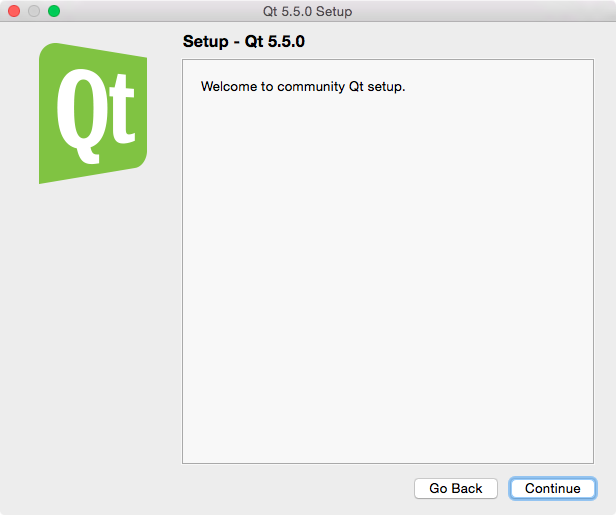
\includegraphics[width=11.5cm]{qt-1}
\caption{Asistente de instalación de Qt~5.5: Página de bienvenida}
\label{fig:qt-1}
\end{figure}

\begin{figure}[htbp]
\centering
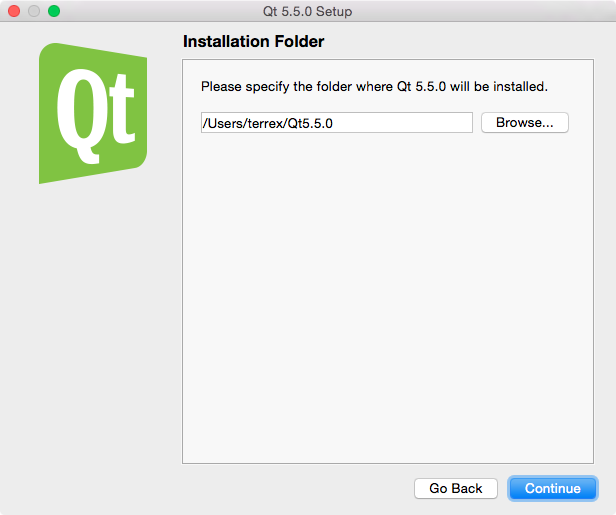
\includegraphics[width=11.5cm]{qt-2}
\caption{Selección de ruta de instalación de Qt}
\label{fig:qt-2}
\end{figure}

\begin{figure}[htbp]
\centering
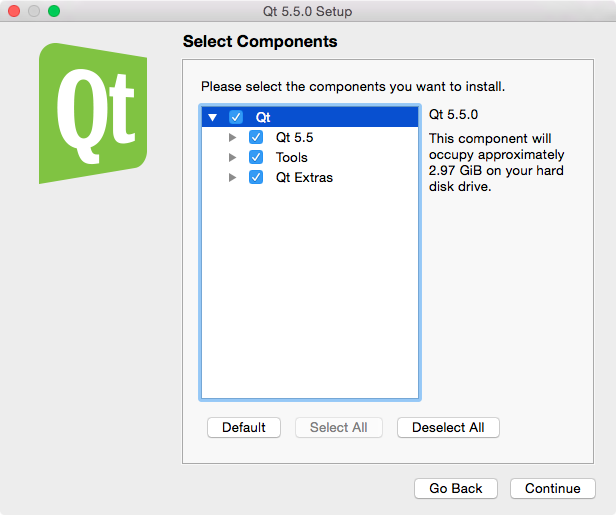
\includegraphics[width=11.5cm]{qt-3}
\caption{Seleccionar todos los componentes para instalar}
\label{fig:qt-3}
\end{figure}

\begin{figure}[htbp]
\centering
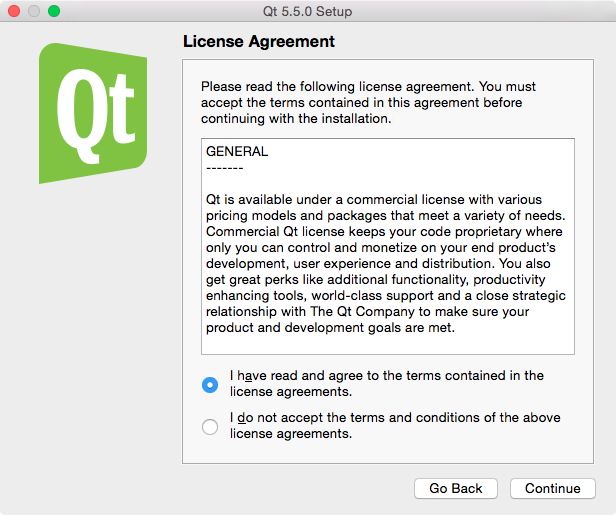
\includegraphics[width=11.5cm]{qt-4}
\caption{Aceptación de licencia}
\label{fig:qt-4}
\end{figure}

\begin{figure}[htbp]
\centering
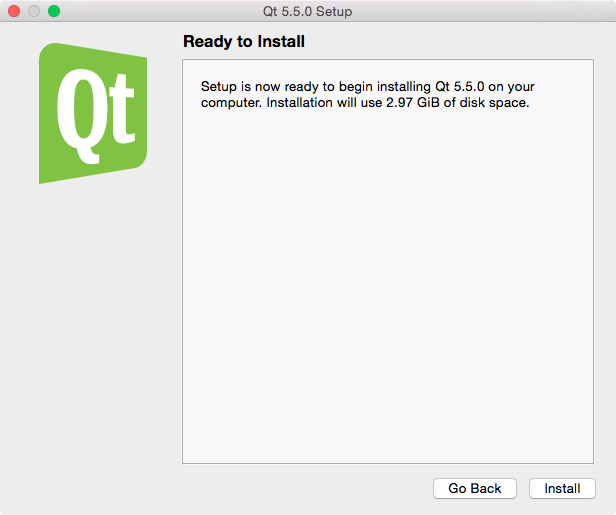
\includegraphics[width=11.5cm]{qt-5}
\caption{Inicio de instalación}
\label{fig:qt-5}
\end{figure}

\begin{figure}[htbp]
\centering
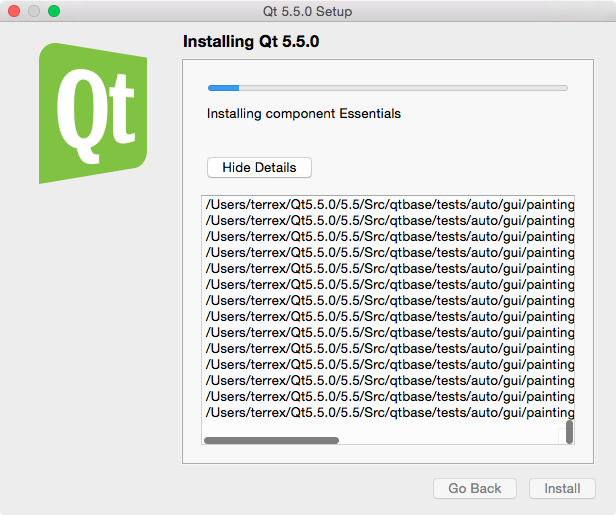
\includegraphics[width=11.5cm]{qt-6}
\caption{Progreso de instalación}
\label{fig:qt-6}
\end{figure}

\begin{figure}[htbp]
\centering
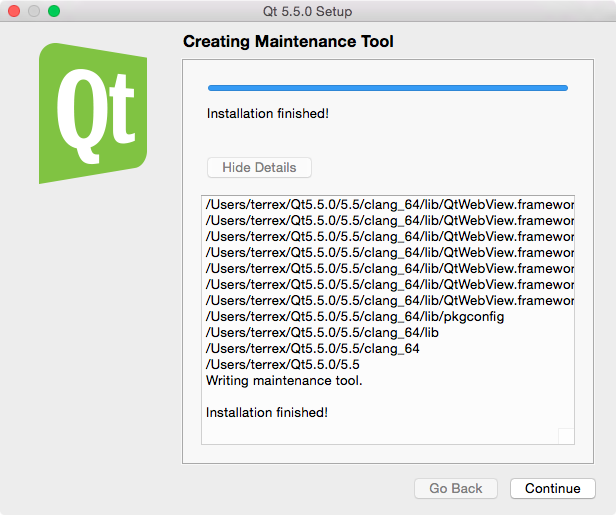
\includegraphics[width=11.5cm]{qt-7}
\caption{Instalación completada}
\label{fig:qt-7}
\end{figure}

\begin{figure}[htbp]
\centering
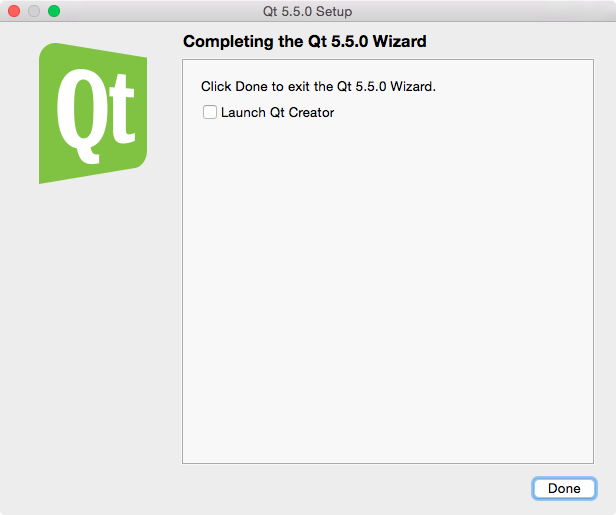
\includegraphics[width=11.5cm]{qt-8}
\caption{Finalización del asistente de instalación de Qt~5.5}
\label{fig:qt-8}
\end{figure}


\subsection{Python~3.4}

Python se encuentra actualmente en dos ``sabores'', versión 2 y versión 3, incompatibles entre sí. En este proyecto nos decantamos por usar el más moderno, y al momento de terminarse el proyecto, la versión concreta que se ha utilizado es Python~3.4.3, aunque debería funcionar en cualquier 3.4.x

Descargar la versión apropiada para su sistema operativo desde la dirección oficial \url{https://www.python.org/downloads/} y seguir las instrucciones del asistente de instalación o de las instrucciones de instalación de la documentación. En el caso de sistemas Mac~OS~X y Windows, se proporciona un asistente de instalación de los binarios; sin embargo para sistemas GNU/Linux se ofrece el paquete del código fuente de Python~3.4.3 listo para compilar.

Otra opción para usar en linux, es utilizar el intérprete Python de su distribución, si es que ésta proporciona alguna versión 3.4, incluyendo el módulo de entornos virtuales \path{venv} y el gestor de paquetes de Python \path{pip} (en Ubuntu son los paquetes \codet{python3-all-dev}, \codet{python3-venv} y \codet{python3-pip}).

\section{Instalación de bibliotecas}

A partir de este momento, tendremos disponibles en la consola el comando de Qt \path{qmake}, y los de Python \path{python3}, \path{pyvenv-3.4} y \path{pip3}.

Es necesario instalar los paquetes de desarrollo. En el caso de Mac~OS~X, la última versión de Xcode; y para Ubuntu, los paquetes listados en el \fullref{lst:ubuntu-apt-get}.

\begin{listing}[htbp]
\begin{minted}{bash}
$ sudo apt-get install ubuntu-dev-tools build-essential \
                       python3-all-dev python3-venv python3-pip \
                       xorg-dev libgl1-mesa-dev libglu1-mesa-dev \
                       libopenblas-dev
\end{minted}
\caption{Paquetes adicionales en Ubuntu}
\label{lst:ubuntu-apt-get}
\end{listing}

\FloatBarrier

Necesitamos las siguientes bibliotecas:
\begin{enumerate}
\item El generador de código \nombrebf{SIP} de Riverbank para la correcta compilación de PyQt5.
\item El \emph{binding} o adaptador de Qt5 para Python llamado \nombrebf{PyQt5} de Riverbank.
\item Los paquetes de pip listados en \blackdirectory{project/requirements.txt}
\end{enumerate}

Los programas de Riverbank pueden descargarse de la página oficial (se pueden probar con versiones futuras sin ningún miedo a perder la compatibilidad hacia atrás):
\begin{itemize}
\item \url{https://riverbankcomputing.com/software/pyqt/download5},\\
archivo \path{PyQt-gpl-5.5.tar.gz}
\item \url{https://www.riverbankcomputing.com/software/sip/download},\\
archivo \path{sip-4.16.9.tar.gz}
\end{itemize}

El primer paso es crear un entorno virtual de Python para evitar conflictos con otras aplicaciones en Python, como paso preventivo, y sin necesidad de tener permisos de superusuario (\autoref{lst:pyvenv}).

\begin{listing}[htbp]
\begin{minted}{bash}
$ pyvenv-3.4 --clear py34
$ source py34/bin/activate
(py34) $ pip3 install -U pip
\end{minted}
\caption[Creación del entorno virtual (pyvenv)]{Creación del entorno virtual (pyvenv), activación y actualización local de \path{pip}}
\label{lst:pyvenv}
\end{listing}
\FloatBarrier

Una vez completado, compilamos e instalamos \path{sip} (\autoref{lst:sip}).

\begin{listing}[htbp]
\begin{minted}{bash}
(py34) $ tar xzf sip-4.16.9.tar.gz
(py34) $ cd sip-4.16.9
(py34) $ python3.4 configure.py
(py34) $ make
(py34) $ make install
(py34) $ cd ..
\end{minted}
\caption{Compilación e instalación de SIP}
\label{lst:sip}
\end{listing}
\FloatBarrier

Después de la instalación de \path{sip}, procedemos a instalar el binding. Nos hemos encontrado un bug en Qt~5.5.0, y necesitamos aplicar un parche previo (\autoref{lst:parche}).

\begin{listing}[htbp]
\begin{minted}{diff}
--- PyQt-gpl-5.5/configure.py   2015-08-07 12:49:40.000000000 +0200
+++ PyQt-gpl-5.5/configure.py   2015-08-07 12:47:23.000000000 +0200
@@ -697,7 +697,7 @@
         lines = f.read().split('\n')
         f.close()
 
-        self.qt_licensee = lines[0]
+        self.qt_licensee = 'Open Source'
         self.qt_shared = (lines[1] == 'shared')
         self.pyqt_disabled_features = lines[2:-1]
 
\end{minted}
\caption[Corrección de bug en Qt~5.5.0]{Corrección de bug en Qt~5.5.0 (\path{PyQt-gpl-5.5-fix-license-typo.diff})}
\label{lst:parche}
\end{listing}
\FloatBarrier

\newpage
Configuramos e instalamos PyQt5 (\autoref{lst:pyqt5}).

\begin{listing}[htbp]
\begin{minted}{bash}
(py34) $ tar xzf PyQt-gpl-5.5.tar.gz
(py34) $ patch -p0 < PyQt-gpl-5.5-fix-license-typo.diff
(py34) $ cd PyQt-gpl-5.5
(py34) $ python3.4 configure.py --qmake ~/Qt5.5.0/5.5/*/bin/qmake
(py34) $ make
(py34) $ make install
(py34) $ cd ..
\end{minted}
\caption{Compilación e instalación de PyQt5}
\label{lst:pyqt5}
\end{listing}
\FloatBarrier

Como último paso, instalamos los paquetes listados como dependencias en el fichero \path{requirements.txt} (\autoref{lst:pip-requirements-txt}).

\begin{listing}[htbp]
\begin{minted}{bash}
(py34) $ pip3 install -U -r project/requirements.txt
(py34) $ python3.4 -m nltk.downloader all
\end{minted}
\caption{Instalación de paquetes de \codet{pip} de dependencias}.
\label{lst:pip-requirements-txt}
\end{listing}
\FloatBarrier

\section{Inicio del programa}

Para iniciar la ejecución del programa, se puede hacer como se indica en el \autoref{lst:start-pfcsamr}.

\begin{listing}[htbp]
\begin{minted}{bash}
(py34) $ cd project
(py34) $ PYTHONPATH=. pfcsamr/gui.py
\end{minted}
\caption{Inicio del programa}.
\label{lst:start-pfcsamr}
\end{listing}
\FloatBarrier


\chapter{Manual de usuario}

\epigraph{``Los ordenadores son buenos siguiendo instrucciones, no leyendo tu mente.''}{\textsc{Donald Knuth} (1938--)}

\section{Carga del fichero de entrenamiento}

La primera pantalla que se muestra al abrir la aplicación es la pestaña de carga (\autoref{fig:ss-01-load-tab}).

\begin{figure}[H]
\centering
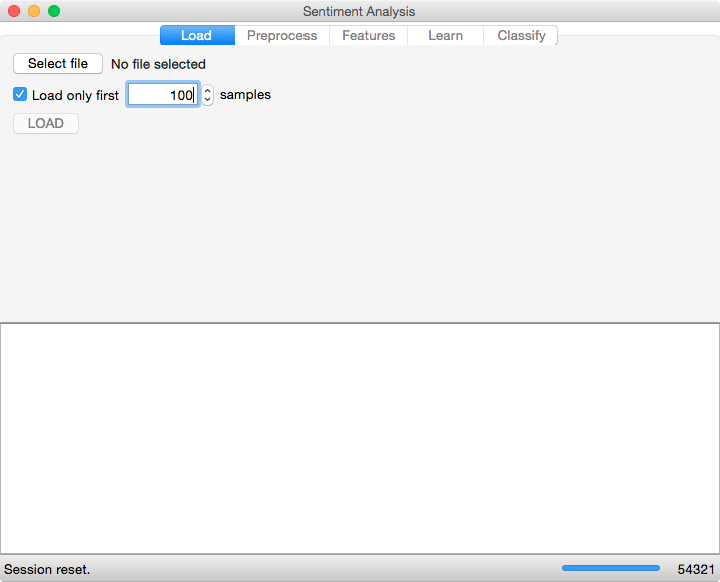
\includegraphics[width=13cm]{ss-01-load-tab}
\caption{Pantalla de carga del fichero de entrenamiento}
\label{fig:ss-01-load-tab}
\end{figure}

\newpage
Al pulsar sobre el botón \menu{Select file} aparece un cuadro de diálogo que permite seleccionar el fichero \path{train.tsv} de entrenamiento (\autoref{fig:ss-02-load-file}).

\begin{figure}[H]
\centering
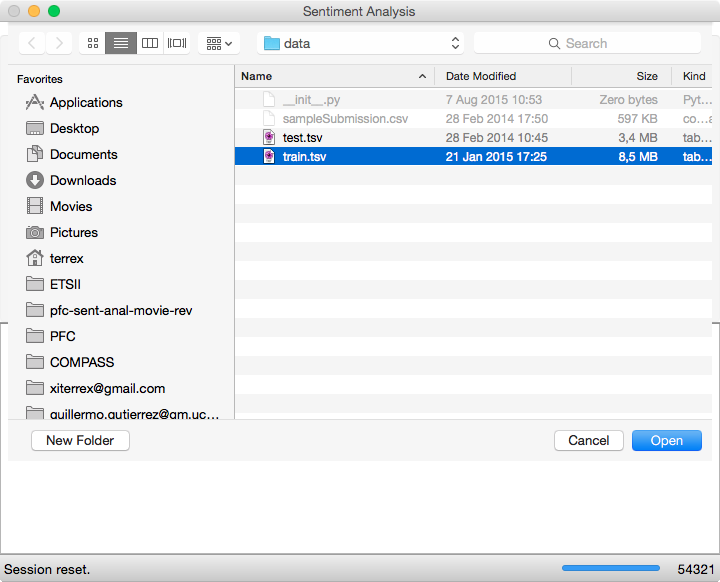
\includegraphics[width=14cm]{ss-02-load-file}
\caption{Pantalla de selección del fichero de entrenamiento}
\label{fig:ss-02-load-file}
\end{figure}

\newpage
Una vez seleccionado, marcar la opción de carga parcial si se desea, indicando el número de muestras. A continuación, pulsar el botón \menu{LOAD}, con lo que aparece el fichero en forma de tabla en el panel de datos (\autoref{fig:ss-03-file-loaded}).

\begin{figure}[H]
\centering
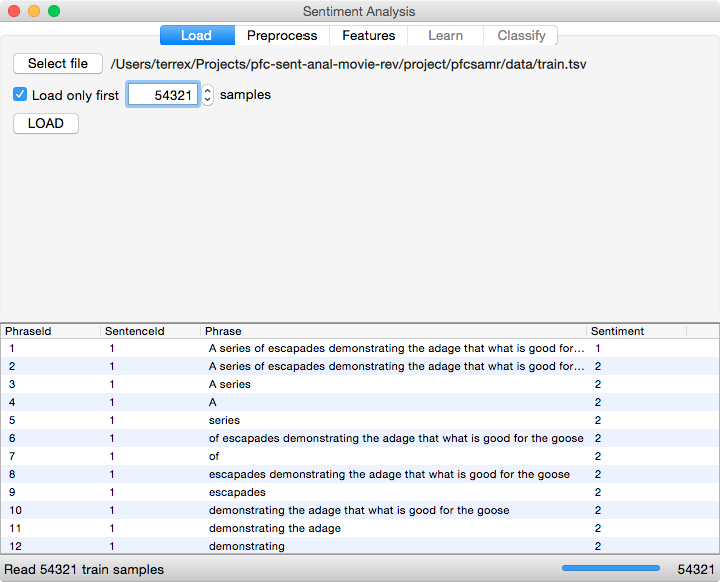
\includegraphics[width=14cm]{ss-03-file-loaded}
\caption{Pantalla con el fichero de entrenamiento cargado}
\label{fig:ss-03-file-loaded}
\end{figure}

\newpage
\section{Opciones de preprocesamiento de texto}
\label{sec:manual-preproc}

Una vez cargado, pasamos a la siguiente pestaña de opciones de preprocesamiento. En esta pantalla, marcamos las opciones deseadas, y a continuación pulsamos el botón \menu{RUN} para proceder al preprocesamiento. Se muestra una barra de progreso a la derecha de la barra de estado, y al terminar, se actualiza el panel de datos con las muestras preprocesadas (\autoref{fig:ss-04-preproc-tab}).

\begin{figure}[H]
\centering
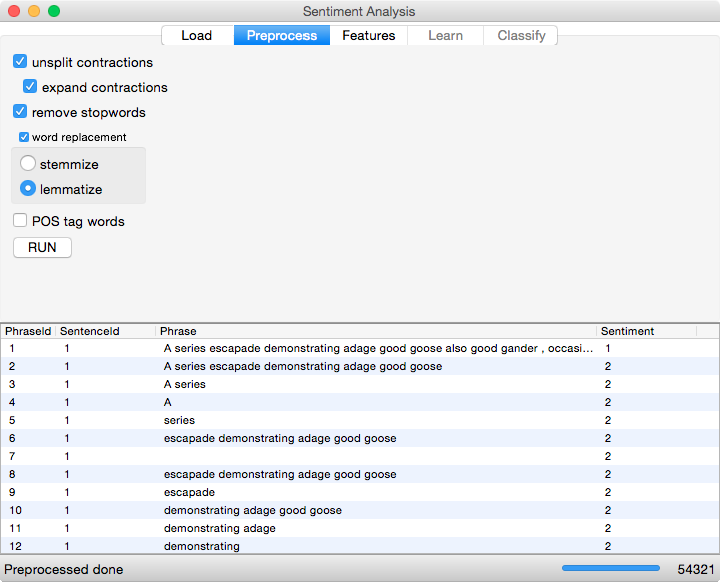
\includegraphics[width=14cm]{ss-04-preproc-tab}
\caption{Pantalla de opciones de preprocesamiento}
\label{fig:ss-04-preproc-tab}
\end{figure}

\newpage
\section{Extracción de características}
\label{sec:manual-features}

El siguiente paso es la extracción de características. Pulsar en la pestaña y marcar las opciones deseadas para la extracción de n-gramas y su reducción. Pulsar en el botón \menu{RUN} para proceder con la transformación. Al finalizar, se muestra el panel de datos con una característica en cada columna, y su valor para cada muestra. El encabezado de la columna indica el n-grama concreto (\autoref{fig:ss-05-feat-tab}).

\begin{figure}[H]
\centering
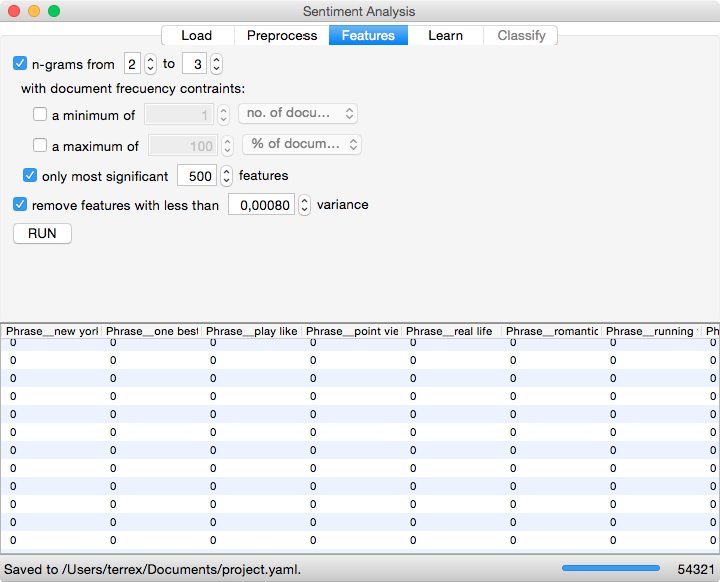
\includegraphics[width=14cm]{ss-05-feat-tab}
\caption{Pantalla de opciones de extracción de características}
\label{fig:ss-05-feat-tab}
\end{figure}

\newpage
\section{Aprendizaje automático del modelo}
\label{sec:manual-learn}

A continuación, avanzamos de pestaña para las opciones de aprendizaje. Se recomienda dejar marcado la división del conjunto en subconjunto de entrenamiento y subconjunto de autoevaluación, para poder obtener una puntuación del modelo aprendido.

Elegir el modelo concreto en la segunda fila de pestañas y pulsar el botón \menu{RUN}. Cuando finalice el aprendizaje, se actualizará el valor de la puntuación (etiqueta \codet{SCORE: }). Hay cinco modelos a elegir, no es obligatorio entrenarlos todos, pero está bien hacerlo para comparar su puntuación y elegir el mejor.

Se puede repetir tantas veces como se desee e ir alterando los parámetros para encontrar la mayor puntuación (\autoref{fig:ss-06-learn-tab}).

\begin{figure}[H]
\centering
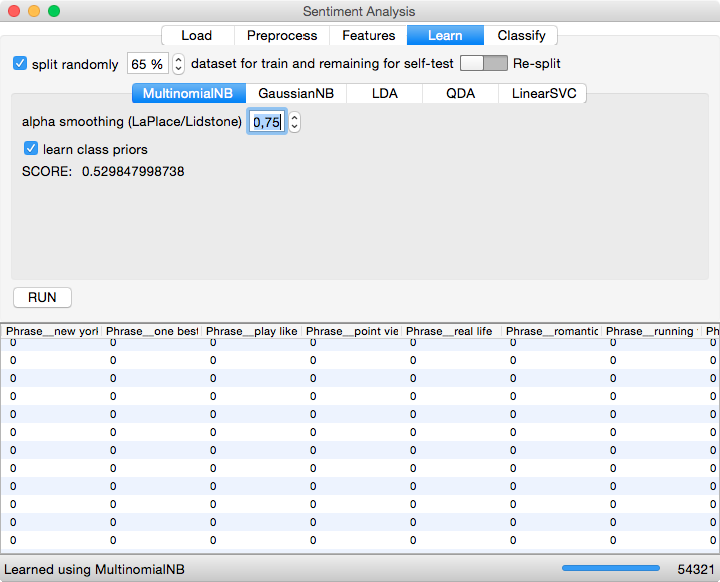
\includegraphics[width=14cm]{ss-06-learn-tab}
\caption{Pantalla de aprendizaje (\codep{MultinomialNB})}
\label{fig:ss-06-learn-tab}
\end{figure}

\newpage
\section{Clasificación del conjunto de clasificación}

Una vez entrenado alguno de los modelos, avanzar pulsando la pestaña siguiente (\autoref{fig:ss-07-classify-tab}). Pulsar el botón \menu{Select file} para elegir el fichero \path{test.tsv} de evaluación.

\begin{figure}[H]
\centering
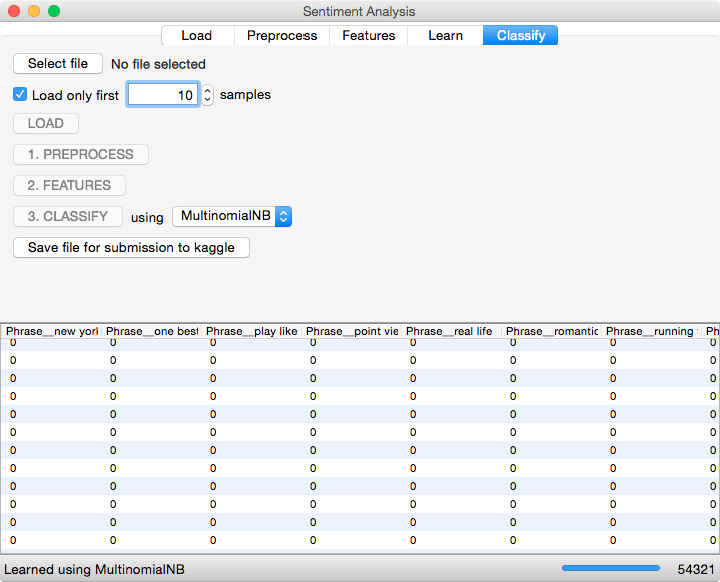
\includegraphics[width=14cm]{ss-07-classify-tab}
\caption{Pantalla de la pestaña de clasificación}
\label{fig:ss-07-classify-tab}
\end{figure}

\newpage
Se puede activar la opción de carga parcial e indicar el número de muestras, si se desea. A continuación pulsar \menu{LOAD} para realizar la carga y la visualización en el panel de datos (\autoref{fig:ss-08-classify-test-loaded}).

\begin{figure}[H]
\centering
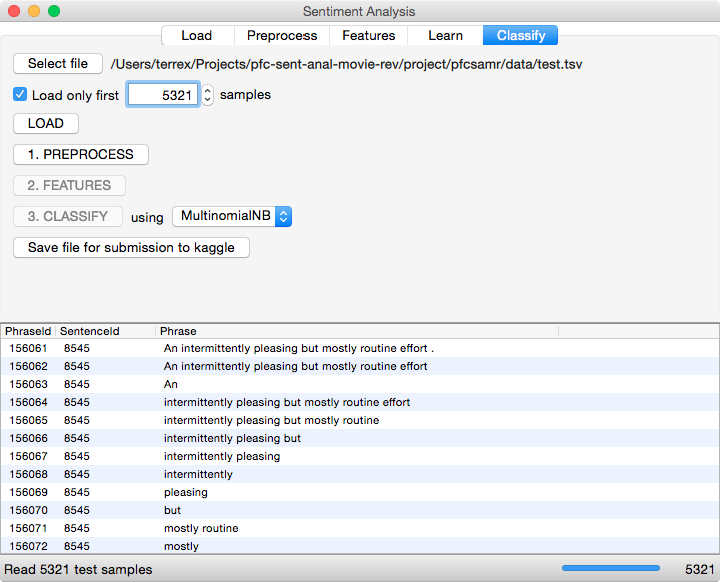
\includegraphics[width=14cm]{ss-08-classify-test-loaded}
\caption{Pantalla con el conjunto de clasificación cargado}
\label{fig:ss-08-classify-test-loaded}
\end{figure}

\newpage
Pulsando el botón \menu{1. PREPROCESS} se realiza el preprocesamiento de texto de clasificación de manera análoga a como se preprocesó el texto de entrenamiento en la fase de entrenamiento (\autoref{sec:manual-preproc}). Se actualizará el panel de datos con el resultado (\autoref{fig:ss-08-classify-test-loaded}).

\begin{figure}[H]
\centering
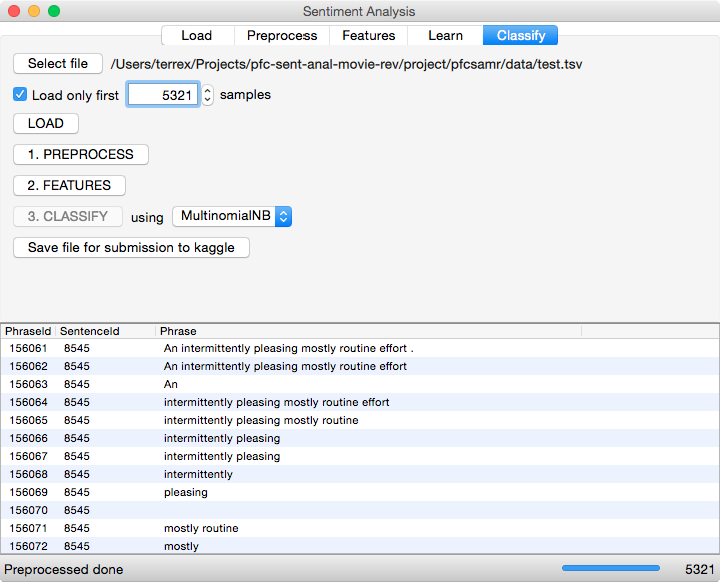
\includegraphics[width=14cm]{ss-09-classify-test-preproccesed}
\caption{Pantalla con el texto preprocesado}
\label{fig:ss-09-classify-test-preproccesed}
\end{figure}

\newpage
Siguiendo con el procedimiento, pulsamos el botón \menu{2. FEATURES} para extraer las características del texto de clasificación preprocesado, que se realiza automáticamente de manera análoga a como se hizo en la fase de entrenamiento (\autoref{sec:manual-features}). Al terminar, se muestra en el panel de datos las características de las muestras a clasificar (\autoref{fig:ss-10-classify-test-featured}).

\begin{figure}[H]
\centering
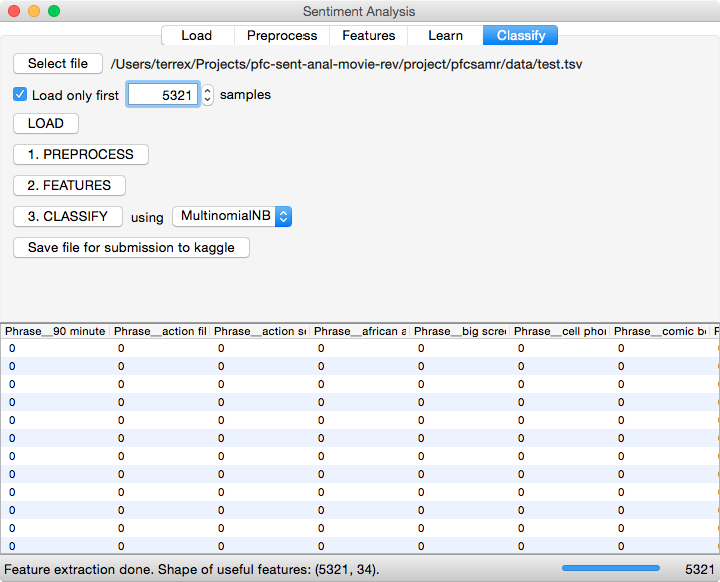
\includegraphics[width=14cm]{ss-10-classify-test-featured}
\caption{Pantalla de características}
\label{fig:ss-10-classify-test-featured}
\end{figure}


\newpage
El último paso es realizar las predicciones. Para ello, elija un modelo del cuadro desplegable. Este modelo debería haber sido entrenado previamente en el paso de entrenamiento (\autoref{sec:manual-learn}), en caso contrario se mostrará un error. Pulsar el botón \menu{3. CLASSIFY} para clasificar las muestras. Aparecerá en el panel de datos las muestras originales con una columna añadida del sentimiento predicho por el modelo seleccionado (\autoref{fig:ss-11-classify-test-predictions}). Si se desea, se puede repetir usando otro modelo.

\begin{figure}[H]
\centering
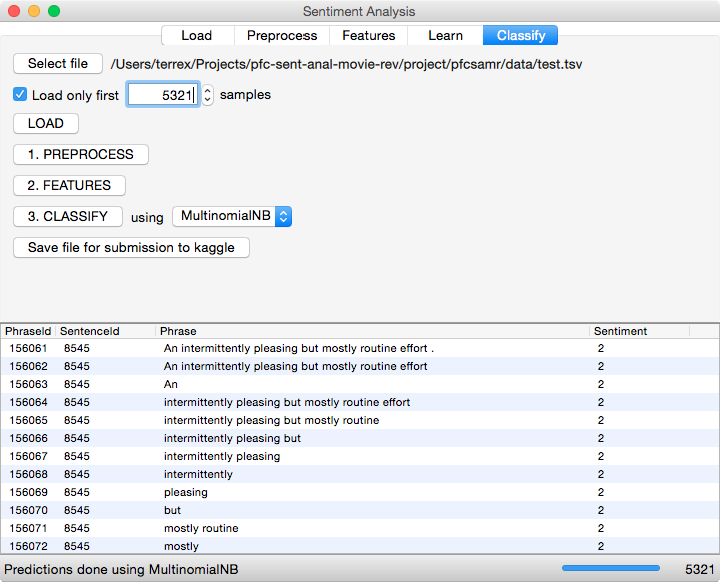
\includegraphics[width=14cm]{ss-11-classify-test-predictions}
\caption{Pantalla con las predicciones de sentimiento}
\label{fig:ss-11-classify-test-predictions}
\end{figure}

Posteriormente, pulsando el botón \menu{Save file for submission to kaggle} se puede guardar el resultado de la clasificación en el formato \path{.csv} para posteriormente entregar en Kaggle.\footnote{\url{https://www.kaggle.com/c/sentiment-analysis-on-movie-reviews}}

\newpage
En cualquier momento, se puede usar el menú \menu{File} para reiniciar el sistema, o abrir o guardar las opciones de la sesión para reanudar posteriormente.

\begin{figure}[H]
\centering
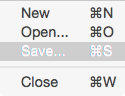
\includegraphics[width=\textwidth]{ss-12-menu-file}
\caption[Pantalla con el menú \codet{FILE}]{Pantalla con el menú \menu{File}}
\label{fig:ss-12-menu-file}
\end{figure}




%% %% %% %% %% %% %%

\backmatter

%% biliografía %%
\nocite{*}
\printbibliography[heading=bibintoc,title=\bibname]

%% índices y tablas %

\cleardoublepage
\phantomsection
\addcontentsline{toc}{chapter}{Índice de tablas}
\listoftables

\cleardoublepage
\phantomsection
\addcontentsline{toc}{chapter}{Índice de figuras}
\listoffigures

\cleardoublepage
\phantomsection
\addcontentsline{toc}{chapter}{Índice de códigos}
\listoflistings

\cleardoublepage
\phantomsection
\addcontentsline{toc}{chapter}{\listSRSActorname}
\listofSRSActor

\cleardoublepage
\phantomsection
\addcontentsline{toc}{chapter}{\listSRSObjname}
\listofSRSObj

\cleardoublepage
\phantomsection
\addcontentsline{toc}{chapter}{\listSRSIrqname}
\listofSRSIrq

\cleardoublepage
\phantomsection
\addcontentsline{toc}{chapter}{\listSRSUcname}
\listofSRSUc

\cleardoublepage
\phantomsection
\addcontentsline{toc}{chapter}{\listSRSNfrname}
\listofSRSNfr

\cleardoublepage
\phantomsection
\addcontentsline{toc}{chapter}{Índice alfabético}
\printindex

\end{document}
